
\section{Introduction} % ================== 

Tobler's First Law of Geography says that things close together in space tend to behave more similarly than things further apart \citep{Tobler1970}. The model fit in Chapter 3 performs well, but we there remains unexplained spatial variation in the mean, and we expect missing covariate information. To account for the unexplained variation and missing covariates, we augment the model with a spatially correlated random effect, giving a Spatial Generalized Linear Mixed Model (SGLMM) \citep{Banerjee2008}.

Broadly speaking, we want to add a spatial random effect to improve our model, and then compare the effectiveness of the SGLMM fit to the GLM fit. More narrowly, as a first step in that process, the research in this chapter examines three procedures and their ability to fit big data SGLMMs on a personal computer (PC). Facilitating access to, and experimentation with, more complex models will encourage research at the amateur, academic, and industrial levels.

This chapter consists of four sections. The first section covers four background topics for the remaining sections: Gaussian Random Fields, SGLMMs, big spatial data computational burdens, and Markov Chain Monte Carlo. The remaining three sections detail three approaches to dealing with the computational burdens of fitting our SGLMM: optimization, dimension reduction, and approximation.

\subsection{Gaussian Random Field} % ================== 

A Gaussian random field (GRF) provides a tractable structure for spatial random effects in a linear model \citep{Gelfand2010}. To define a GRF, first define vector of locations $\pmb{s} \in \pmb{D} \subseteq \pmb{R}^{2}$, for spatial domain $\pmb{D}$. Then, define multivariate Normal random vector $\pmb{w}(\pmb{s})$, with mean $\pmb{0}$; and symmetric, positive definite covariance matrix $\Sigma(\pmb{\theta})$, with covariance parameters $\pmb{\theta}$ \citep{Haran2011}.
\begin{equation} \label{eq:w}
\pmb{w}(\pmb{s}) | \pmb{\theta} \sim MVN(\pmb{0}, \Sigma(\pmb{\theta})) 
\end{equation}
In sections \ref{stanopt} and \ref{ppm} we use a spatial exponential covariance structure for $\Sigma(\pmb{\theta})$. Element $i,j$ of the exponential covariance matrix, $\pmb{\Sigma}(\pmb{\theta})$, gives the covariance of the random effects $\pmb{w}(\pmb{s}_{i})$ and $\pmb{w}(\pmb{s}_{j})$:
\begin{equation} \label{eq:exp}
\Sigma(\phi, \sigma^{2})_{i,j} = \sigma^{2} exp(-||\pmb{s}_{i} - \pmb{s}_{j}||/\phi),
\end{equation}
with scale parameter $\sigma^{2}$, range parameter $\phi$, and where $||s_{i} - s_{j}||$ denotes the Euclidean distance between $\pmb{s}_{i}$ and $\pmb{s}_{j}$. In the next section we define the SGLMM we use.

\subsection{Spatial Generalized Linear Mixed Model}
Adding $\pmb{w}(\pmb{s})$ to the linear predictor in equation \ref{eq:glm} gives the following spatial generalized linear mixed model (SGLMM):
\begin{equation} \label{eq:SGLMM}
\text{logit}(p_{ij}|\pmb{s}_{ij}) = \pmb{X}_{ij}(\pmb{s}_{ij}) \pmb{\beta}_{j} + w(\pmb{s}_{ij}).
\end{equation}

This spatial model, containing a latent (unobserved) Gaussian random field, gives $\pmb{Y}$ a complicated correlation structure. Bayesian hierarchical spatial models most effectively accommodate this structure, and Markov chain Monte Carlo (MCMC) methods most effectively estimate model parameters \citep{Banerjee2014}. High dimensionality for this spatial model induces substantial computational costs, referred to as the ``Big N problem'' \citep{Lindgren2011}. We describe the Big N problem next.

\subsection{Three Approaches to the ``Big N Problem''}

Recall the multivariate Normal probability distribution function, for $\pmb{w}$ in our case.
\begin{equation} \label{eq:mvn}
f(\pmb{w}) = \frac{1}{(2\pi)^{n/2}|\Sigma|^{1/2}} \text{exp}\{ -\frac{1}{2}\pmb{w}'\Sigma^{-1}\pmb{w} \}
\end{equation}
Note that $|\Sigma|^{1/2}$ denotes the square root of the determinant of the n $\times$ n covariance matrix, and $\Sigma^{-1}$ denotes its inverse \citep{Lay}. For large sample sizes, these two components of the MVN distribution lead to prohibitive computational costs. To define the cost, we introduce ``big oh'' notation. 

For a sequence of two increasing functions $f(n)$ and $g(n)$, we say ``$f(n)$ is big `oh' $g(n)$ as n goes to infinity,'' or $f(n) = \mathcal{O}(g(n))$ as $n \rightarrow \infty$, if and only if there exists some $n_{0}$ and a positive real number M such that
  $$|f(n)| \leq \text{M} \cdot |g(n)| \text{ for all } n \geq n_0 $$
The computational costs of fitting a SGLMM with a latent GRF increase at a rate of $\mathcal{O}(n^{3})$ \citep{Finley2009}. We can define t(n) as time required to fit our model type to n observations; then:
$$t(n) \leq M \cdot n^{3} \text{ as } n \rightarrow \infty.$$
In less technical terms, this means the upper bound on the amount of time required for model fitting increases at the same rate as $n^{3}$. To understand why, refer back to the MVN pdf in equation \ref{eq:mvn}, and notice the n $\times$ n covariance matrix inverse and the determinant. Every MCMC algorithm iteration requires calculation and construction of these components; this accounts for the $\mathcal{O}(n^{3})$ rate of increase, prohibitively slow model fitting, and the ``Big N'' problem. 

To address these computational challenges, we tried three model-fitting approaches.
\begin{enumerate}
\item Computational optimization in Bayesian computing software Stan \citep{rstan}.
\item Dimension reduction with Predictive process models, implemented in R with the R package \verb|spBayes| \citep{Eidsvik2012}, \citep{Finley2013}.
\item Integrated Nested Laplace Approximations with Stochastic Partial Differential Equations, implemented in the R with the package \verb|INLA-R| \citep{Lindgren2015}.
\end{enumerate}
The first two approaches rely on the prevalent Bayesian model fitting algorithm  MCMC, the subject of the next section.

\subsection{Markov Chain Monte Carlo}

In Bayesian statistics we seek the posterior distribution of the parameter/s of interest, given the observed data. The fundamental Bayesian proportionality, for observation vector $\pmb{y}$, and parameter vector $\theta$, takes the form \citep{Gelman2014}:
\begin{equation} \label{eq:bayes}
p(\pmb{\theta}|\pmb{y}) \propto f(\pmb{y}|\pmb{\theta})p(\pmb{\theta}).
\end{equation}
Elementary Bayesian models sometimes yield closed form posterior distributions, but more complex models rarely do. For complex models, MCMC offers an iterative procedure that converges to the true posterior distribution. This class of procedures presents its own challenges and weaknesses, but, with sufficient computing power and time, often provides the desired posterior distribution. The MCMC solution presents itself empirically, as samples from the posterior distribution of interest, rather than as a closed form. 

Markov chain properties supply the critical theoretical components of MCMC. Foremost among them, a sequence of possibly multivariate random variables $\pmb{X}_{1}, \pmb{X}_{2}, \hdots \pmb{X}_{n}$ possesses the Markov property if the distribution of $\pmb{X}_{n+1}|\pmb{X}_{1}, \pmb{X}_{2}, \hdots , \pmb{X}_{n}$ depends only on $\pmb{X}_{n}$. A sequence of random variables with the Markov property constitutes a Markov chain. MCMC algorithms use Markov chains that possess additional, necessary technical properties that assure an equilibrium distribution \citep{Brooks2011}. In fact, MCMC chains converge to an equilibrium distribution equivalent to the posterior distribution of interest.

Both Bayesian estimation programs used in this chapter use the Metropolis sampling algorithm, one of the most popular MCMC algorithms. \verb|Stan| uses HMC sampling and a ``Metropolis reject step'' \citep{STANtheMan}; while \verb|spBayes| uses a ``Metropolis-within-Gibbs'' sampler \citep{Finley2013}. 

In the next two sections we describe the Metropolis algorithm and the Gibbs sampler. The Metropolis algorithm manufactures samples from a distribution with a density function only known up to a proportionality constant; while the Gibbs sampler draws, often using the Metropolis, from a sequence of conditional distributions that converges to the posterior distribution of interest.

\subsubsection{Metropolis Algorithm } % \citep{Banerjee2014}

Often we don't have the closed form for a target distribution, such as an MCMC iteration conditional distribution, or the full posterior distribution. However, we always know the target distribution up to a proportionality constant, and thus have the posterior kernel. Let $h(\pmb{\theta})$ denote the posterior distribution kernel. The Metropolis algorithm uses $h(\pmb{\theta})$ to iteratively draw samples from the full conditionals, $p(\theta_{i}|\pmb{\theta}_{-i})$; and essentially reduce a high dimensional problem to a series of lower dimension problems. 

The algorithm requires a  candidate density, $q(\pmb{\theta}_{t}|\pmb{\theta}_{t-1})$, that we can readily draw samples from; whose support contains all possible values of $\pmb{\theta}_{t}$ and $\pmb{\theta}_{t-1}$; and is symmetric, ($q(\pmb{\theta}_{t}|\pmb{\theta}_{t-1}) = q(\pmb{\theta}_{t-1}|\pmb{\theta}_{t})$). Then, for $(t \in 1:T)$, with T prescribed iterations, we choose an initial value $\pmb{\theta}_{0}$ for $\pmb{\theta}$, and the algorithm proceeds as follows.
\begin{enumerate}
\item Generate candidate value of $\pmb{\theta}$, call it $\pmb{\theta}^{*}$, from $q(\pmb{\theta}^{*}|\pmb{\theta}_{t})$.
\item Compute the ratio of kernels,
$$ r=h(\pmb{\theta}^{*})/h(\pmb{\theta}^{t-1}) = \text{exp}[\text{log }h(\pmb{\theta}^{*}) - \text{log }h(\pmb{\theta}^{(t-1)}). $$
\item If $r \geq  1$, set $\pmb{\theta}^{t} = \pmb{\theta}^{*}$; \\
            If $r < 1$, set 
            \[ 
            \pmb{\theta}^{t} = 
            \begin{cases} 
            \pmb{\theta}^{*} \text{ with probability r} \\
            \pmb{\theta}^{(0)} \text{ with probability 1 - r} \\
            \end{cases}
            \]
  \end{enumerate}
This algorithm successfully draws samples from a distribution known only up to a proportionality constant.   

\subsubsection{Gibbs Sampler}
In the now common high dimensional problems, the Gibbs Sampler achieves success, in part, because it iteratively reduces the dimension of the problem. To understand how, and delineate the algorithm, first define parameter vector $\pmb{\theta} = (\theta_{1}, \dots, \theta_{k})'$. We assume here we can draw samples from $p(\theta_{i}|\theta_{j \neq i},y)$ directly, or use the Metropolis algorithm described in the previous section. The Gibbs sampler proceeds with the following steps, for iterations $(t \in 1:T)$ \citep{Banerjee2014}. 
        \begin{itemize} 
        \item Step 1: draw $\theta_{1}^{t}$ from $p \left( \theta_{1}|\theta_{2}^{t-1}, \theta_{3}^{t-1},\dots,\theta_{k}^{t-1},\pmb{y} \right)$ 
        \item Step 2: draw $\theta_{2}^{t}$ from $p \left(\theta_{2}|\theta_{1}^{t}, \theta_{3}^{t-1},\dots,\theta_{k}^{t-1},\pmb{y} \right)$ \\
        $\vdots$
        \item Step k: draw $\theta_{k}^{t}$ from $p \left( \theta_{k}|\theta_{1}^{t}, \theta_{3}^{t},\dots,\theta_{k-1}^{t},\pmb{y} \right)$ 
        \item Repeat for all $(t \in 1:T)$
        \end{itemize} 
If the chain satisfies certain regularity conditions, as it does in MCMC usage, then the iterations converge to samples from the true posterior distribution $p(\pmb{\theta}|\pmb{y})$ \citep{Banerjee2014}. 

In the next section we present our first attempt to address the big N computational problem: optimization techniques in Stan. As mentioned, Stan uses the Metropolis algorithm with an unusual proposal mechanism.

\section{Optimization in Stan} \label{stanopt} % =================

The Metropolis algorithm requires a proposal generating mechanism, such as a proposal distribution. Often a random walk distribution, or some other accessible distribution, plays this role. On the other hand, Stan uses a proposal mechanism that originated in physics, Hamiltonian Monte Carlo (HMC), to generate proposals for the Metropolis reject step. HMC generates well-mixed, high probability proposals---two important factors. Mixing refers to the degree to which proposals explore the parameter space, and acceptance rates refer to the likelihood that the algorithm accepts proposals. Insufficient mixing and low acceptance rates delay, or even prevent, the sampling algorithm from converging to its equilibrium distribution. While an acceptance rate too high signals insufficient mixing and potentially overly correlated draws. In Stan's MCMC, HMC balances the proposal mechanism demands well. 

In the next section we give the origins and a conceptual overview of HMC.

\subsection{Hamiltonian Monte Carlo} 

HMC history unfolded in four stages, to simplify greatly. First, \cite{Metropolis1953} developed MCMC while conducting research into molecular states. Second, much later \cite{Alder1959} introduced {\it Hamiltonian dynamics} as an alternate representation of Newtonian mechanics, while modeling molecular motion as a deterministic process \citep{Newt}. Third, almost 30 years later, \cite{Duane1987} combined the two to create ``hybrid Monte Carlo,'' to simulate quantum mechanical processes. Over time, the name morphed into {\it Hamilton} Monte Carlo (HMC). Fourth, eventually HMC made its way into statistics, when \cite{Neal1996} used HMC to study neural networks.

To understand HMC, imagine a puck with known position and momentum on a frictionless surface, then randomly changing the momentum of the puck to alter its course, and caluclating the new position. HMC treats the variables of interest as position variables, and uses randomly generated auxiliary Gaussian variables to change the momentum. Then, the new position, calculated with a set of differential equations, provides proposals for Metropolis updates. The differential equation solutions estimate trajectories of the hypothetical physical object (the puck), which then occupies a new position after a time step of some chosen duration. This crafty formulation provides distant (well mixed), yet high probability (high acceptance rate) proposals. This contrasts favorably with the random walk proposal generation process commonly used.\footnote{I dedicate this section to my high school physics teacher, the late William T. Meyers. He helped instill in me a love of physics, and emphasized that in his class we would learn critical thinking skills that we could use in our life.}

\subsection{The Hamilton Equations} % =================

To define the Hamilton equations for d variables of interest, let d-dimensional position vector $q(t)$ depend on time $t$; and let $U(q(t))$ denote the potential energy at time $t$. Let $p(t)$ give the d-dimensional momentum at time $t$, and $K(p(t))$ denote kinetic energy at time $t$. Then the Hamilton equation,
\begin{equation}
H(q(t),p(t)) = U(q(t)) + K(p(t)),
\end{equation}
measures the total energy of a system as a function of potential and kinetic energy. 

In HMC applications, we let the potential energy, $U(q)$, be minus the log of the probability density function of interest, plus a constant.\footnote{We omit $t$ for clarity of presentation, here and elsewhere, but position and momentum remain functions of time $t$.} Next, define d-dimensional vector $p$ as a zero mean Gaussian random variable with covariance matrix M, and define $K(p)$ as minus the log of the multivariate Gaussian probability density function. This gives the Hamilton equation form:
\begin{equation} \label{eq:ham}
H(q,p) = -\text{log}f_{q}(q) + p^{T}\pmb{M}^{-1}p/2.
\end{equation}
This formulation yields tractable partial derivatives for calculating the change in position and momentum through time. For $i = 1,\dots, \text{d}$:
\begin{align}
\frac{d q_{i}(t)}{dt} &= \frac{\partial H}{\partial p_{i}}, \\
\frac{d p_{i}(t)}{dt} &= -\frac{\partial H}{\partial q_{i}}.
\end{align}
Substituting equation \ref{eq:ham} and simplifying gives:
\begin{align}
\frac{d q_{i}(t)}{dt} &=  [\pmb{M}^{-1}p]_{i} \\
\frac{d p_{i}(t)}{dt} &= \frac {\partial \left[ \text{log}f_{q}(q) \right]}{\partial q_{i}}
\end{align}
The differential equation solutions give the position and momentum at time t. With solutions in hand, the ``leapfrog method'' calculates changes in the Hamilton through small time steps, by discretizing the continuously defined Hamilton equation using Taylor Series approximations \citep{Neal2011}. 

In summary, the HMC algorithm samples from the auxiliary Normal distribution, and then calculates the proposal as the positions vector in the Hamilton equation. This method yields high probability, well mixed Metropolis proposals. This combination, and Stan's reputation for efficient Bayesian model fitting, motivated us to use Stan for model fitting. The next section describes techniques specific to Stan, for fast, efficient model fitting. 

\subsection{Optimization Techniques} % =================
With the techniques presented in this section, we aimed to improve Stan model fitting efficiency enough to successfully fit our SGLMM to thousands, or tens of thousands, of observations. The techiques include Bayesian, linear algebra, and purely computational strategies. We start with techniques related to the Bayesian model components.

Stan permits users to omit prior distributions for parameters, but then assumes a non-informative, uniform prior for that parameter. However, prominent Bayesian statistician and Stan developer Andrew Gelman pointed out in personal correspondence that the exponential covariance range parameter, $\phi$ in equation \ref{eq:exp}, requires an informative prior for model identifiability (uniqueness) \citep{Gelman2014}. In this vein, Stan developer Rob Trangucci recommended, also in personal correspondence, a sharp tailed prior distribution for range parameter $\phi$, such as the normal or log-normal, to act as soft upper and lower bound constraints \citep{Trangucci}. Even further, for practical computing time and convergence considerations, Trangucci indicated complex models---such as spatial hierarchical models---require proper priors for all $\beta$ coefficients \citep{Trangucci}. The next two techniques combine linear algebra and computational considerations.

For all operations in Stan, matrix algebra and vectors acheive greater speed and efficiency than loops and scalars \citep{STANtheMan}. For example, 
\begin{verbatim}
hit ~ bernoulli_logit(X*beta + Z)
\end{verbatim}
runs faster than
\begin{verbatim}
for (n in 1:N)
        hit[n] = bernoulli_logit(X[n]*beta[n] + Z[n])
\end{verbatim}
The first, faster line includes N$\times$1 column vectors \verb|hit|, \verb|beta|, and \verb|Z|; and N$\times$p matrix \verb|X|. The second, slower snippet, instead uses scalars \verb|hit[n]|, \verb|beta[n]|, and \verb|Z[n]|; and 1$\times$p row vector \verb|X[n]|.

Trangucci also suggested a QR factorization on covariate matrix $\pmb{X}$, in the linear predictor, to increase computational efficiency \citep{Trangucci}. A QR factorization consists of factoring an n $\times$ p matrix into the product of an n $\times$ p orthogonal matrix $\pmb{Q}$ and a p $\times$ p upper triangular matrix $\pmb{R}$, such that $\pmb{X} = \pmb{QR}$. Leveraging this factorization into a speed increase requires a reparameterization. To this end, let $\pmb{\theta} = \pmb{R \beta}$, which gives:
\begin{align}
\pmb{X} &= \pmb{QR} \\
\pmb{X \beta} &= \pmb{QR \beta} \\
\pmb{X \beta} &= \pmb{Q \theta},
\end{align}
and the model
\begin{equation} \label{eq:reparam}
\text{logit}(p_{ij}|\pmb{s}_{ij}) = \pmb{Q}_{ij}(\pmb{s}_{ij}) \pmb{\theta}_{j} + w_{ij}.
\end{equation}
With this parameterization we incorporate prior information about $\pmb{\beta}$ in the $\pmb{\theta}$ prior distributions. 

Consider non-informative prior distributions on p-dimensional parameter vector $\pmb{\beta}$,
\begin{equation}
\pmb{\beta} \sim N(\pmb{0}, \sigma^{2}\pmb{I}_{p}), 
\end{equation}
with p $\times$ p identity matrix $\pmb{I}_{p}$; and p $\times$ 1 zero vector $\pmb{0}$. Notice the intended variance of the non-informative prior must be modified, to be on the scale of $\pmb{\theta}$.
\begin{align}
\text{Var}(\pmb{\theta}) &= \text{Var}(\pmb{R \beta}) \\
&= \pmb{R}\text{Var}(\pmb{\beta})\pmb{R}' \\
&= \pmb{R}\sigma^{2}\pmb{I}_{p}\pmb{R}' \\
&= \sigma^{2} \pmb{R}\pmb{R}'
\end{align}
This essential follow-up adjustment ensures appropriate weighting of prior information. Next, we look at a purely computational modification.

While we chose a covariance structure meeting all necessary criteria, we add computational noise to the covariance matrix diagonal, with the following snippet of code, to ensure {\it numerical} positive-definiteness.
\begin{verbatim}
for (n in 1:N)
  Sigma[n, n] = Sigma[n, n] + 1e-6;
\end{verbatim}
The stan function \verb|cov_exp_quad(...)| assembles the covariance matrix, and the added diagonal noise guarantees that it remains numerically positive-definite \citep{Trangucci2017}. This reduces wasted MCMC iterations, because \verb|cov_exp_quad(...)| can generate numerically non-positive-definite matrices when operating at high dimensions.

Finally, Stan developer Bob Carpenter recommended, in personal communication, a Cholesky decomposition and reparameterization, noting the efficiency of a vectorized scalar approach \citep{Carpenter}.
\begin{verbatim}
L = cholesky_decompose(Sigma);  
Z ~ normal(0, 1);  
Z_mod = L * Z; 
hit ~ bernoulli_logit(Q*theta + Z_mod);
\end{verbatim}
The first line performs a Cholesky decomposition on the covariance matrix \verb|Sigma|, by finding lower triangular matrix \pmb{L} such that $\Sigma = \text{\pmb{LL}}'$. Line 2, ``vectorized scalar'' \verb|Z ~ normal(0, 1)| generates n standard normal random variables, by reusing ``\verb|normal(0, 1)|'' for every element of \verb|Z|. These two lines remove the dependence of random vector \pmb{Z}, which must be generated, on the unknown parameters \citep{Trangucci2017}. The third line, \verb|Z_mod = L * Z|, uses \verb|L| to transform \verb|Z|, so that \verb|Z_mod| possesses the desired distribution. Note that $\text{Var}(\text{\pmb{LZ}}) = \text{\pmb{L}} \text{I}_{n}\text{\pmb{L}}' = \Sigma$, so that $\pmb{LZ} \sim N(\pmb{0}, \Sigma)$ as desired. The final line specifies the model.

This collection of techniques improved the model fit efficiency somewhat, which we discuss in the next section.

\subsection{Results}

In initial model fitting, using a test data set of n = 25 observations, to sample one 500 sample chain required approximately 50 seconds of computing time. Using the Cholesky decomposition described above reduced this time to 26 seconds. Proper priors on covariance parameters and noise on the covariance diagonal drastically reduced the number of numerical/sampling errors and warning messages, shaving another few seconds off the computing time. Using proper, non-informative priors for all elements of $\pmb{\beta}$ reduced computing time for n=25 observations to approximately 5 seconds. 

However, increasing the number of observations to n=500 required approximately 100 minutes; increasing the observations by a factor of 20 increased the computing time by a factor of 1200. The $\pmb{QR}$ decomposition yielded significant further gains: n = 1000 observations required about 60 minutes. As a point of reference, fitting a GLM---without a spatial random effect---with the same number of observations required about six {\it seconds}. Despite these improvements, Stan-based modeling efforts ended at n = 2000, when an overnight MCMC fit attempt yielded only 350 of 500 samples.

Optimization in Stan proved inadequate for addressing the ``big N'' problem. Next, in an effort to address the big N problem in another way, we examine an approach that creates a reduced dimension representation of a SGLMM. 

\section{Dimension Reduction with Predictive Process Models} \label{ppm} % ======

\subsection{Introduction}

Predictive process models (PPMs) reduce the dimension of our SGLMM's covariance matrix to circumvent the big N problem. Several general strategies exist for this task, with often several methods to implement each strategy. \cite{Fuentes2007} and \cite{Paciorek2007} use a spectral representation of the covariance function, and Fourier transformations, to reduce the dimensionality of data on a regular lattice. ``Covariance tapering'' involves setting small values in the covariance matrix to zero, and achieving computational gains that come with a sparse matrix \citep{Furrer2006}, \citep{Kaufman2008}. We explore one computational approximation approach in Section \ref{INLA} \citep{Rue2009}, but others exist \citep{Stein2004}, \citep{Eidsvik2014}, \citep{Aune2014}. Still others approaches, including PPMs which we use, apply exact methods to a simplified, lower rank version of the original model \citep{Cressie2008}, \citep{Higdon2002}, \citep{Eidsvik2012}.

PPMs provide a competitive modeling approach, and computational advantages specific to hierarchical models with a GRF at the second level of specification---such as our SGLMM \citep{Banerjee2008}. Gaussian PPMs project the original spatial process onto a lower dimensioned subspace, at a set of locations called knots, to achieve dimension reduction \citep{Banerjee2008}. In the next section we describe this procedure in detail, defining additional notation as necessary.

\subsection{PPM Procedure}
Consider again the SGLMM from equation \ref{eq:SGLMM}, defined as it was there, and Gaussian random field $\pmb{w}(\pmb{s})$:
\begin{align}
\text{logit}(p_{ij}|\pmb{s}_{ij}) &= \pmb{X}_{ij}(s_{ij}) \pmb{\beta}_{j} + w(\pmb{s}_{ij}) \label{eq:ppm} \\
\pmb{w}(\pmb{s}) | \pmb{\theta} &\sim \text{GRF}(\pmb{0}, \pmb{C}(\pmb{\theta})) \label{eq:GRF}
\end{align}
Equation \ref{eq:GRF} defines a stationary GRF for n $\times$ 1 vector of random effects $\pmb{w}$, at locations $\pmb{s}$, conditioned on covariance parameters $\pmb{\theta}$; with mean  n $\times$ 1 zero vector $\pmb{0}$; and a symmetric, positive-definite, n $\times$ n covariance matrix $\pmb{C}(\pmb{\theta})$.

To begin to define the PPM procedure, let $C(\pmb{s}_{i}, \pmb{s}_{j}; \pmb{\theta})$ denote the covariance of random effects at locations $\pmb{s}_{i}$ and $\pmb{s}_{j}$, so that $C(\pmb{\theta}) = [C(\pmb{s}_{i}, \pmb{s}_{j}; \pmb{\theta})]_{i,j=1}^{n}$. Next, let $\pmb{S}^{*} = \{\pmb{s}_{1}^{*}, \dots, \pmb{s}_{m}^{*}\}$ give a set of $m << n$ chosen knot locations, not necessarily a subset of observed locations.\footnote{Knot selection is equivalent to the area of study known as spatial sampling design \citep{Finley2009}. See \citep{Xia2006} for a summary of spatial sampling approaches.} We denote knot location random effects with m $\times$ 1 vector $\pmb{w}^{*} = \left[w(\pmb{s}_{i}^{*})\right]_{i=1}^{m}$, and the m $\times$ m knot covariance matrix and its elements as $\pmb{C}^{*}(\pmb{\theta}) = \left[C(\pmb{s}_{i}^{*}, \pmb{s}_{j}^{*})\right]_{i,j = 1}^{m}$. The knot random effects constitute a distinct m-dimensional GRF:
\begin{equation}
\pmb{w}^{*}|\pmb{\theta} \sim \text{GRF}\{\pmb{0}, \pmb{C}^{*}(\pmb{\theta})\}.
\end{equation}

Consider a new loction $\pmb{s}_{0}$. The PPM procedure uses the m knots, the covariance structure of the parent process, and kriging to interpolate $w$ at $\pmb{s}_{0}$ \citep{Schabenberger2004}. To see this, let $\tilde{w}(\pmb{s}_{0})$ represent this interpolated random effect, and let $\pmb{c}(\pmb{s}_{0};\pmb{\theta}) = \left[C(\pmb{s}_{0}, \pmb{s}_{j}^{*}; \pmb{\theta})\right]_{j = 1}^{m}$ be an m $\times$ 1 covariance vector giving the covariance of the $\pmb{s}_{0}$ random effect with the knot random effects. Then,  kriging estimator
\begin{align}
\tilde{w}(\pmb{s}_{0}) &= E[w(\pmb{s}_{0})|\pmb{w}^{*}] \\ 
&= \pmb{c}^{T}(\pmb{s}_{0};\pmb{\theta}) \cdot \pmb{C}^{*-1}(\pmb{\theta}) \cdot \pmb{w}^{*} \label{eq:krig}
\end{align}
minimizes the squared error loss function among all linear predictors \citep{Schabenberger2004}. Notice that the linear combination (\ref{eq:krig}) varies spatially. Accordingly, predictive process $\tilde{w}(\pmb{s})$ defines the following GRF and covariance matrix.
\begin{align}
\tilde{\pmb{w}}(\pmb{s}) &\sim \text{GRF}\{0, \tilde{C}(\cdot)\} \\
\tilde{C}(\pmb{s}, \pmb{s}'; \pmb{\theta}) &= \pmb{c}^{T}(\pmb{s};\pmb{\theta}) \cdot \pmb{C}^{*-1}(\pmb{\theta}) \cdot \pmb{c}(\pmb{s}';\pmb{\theta})
\end{align}
Recall m $\times$ 1 vector $\pmb{c}(\pmb{s};\pmb{\theta}) = \left[C(\pmb{s}, \pmb{s}_{j}^{*})\right]_{j = 1}^{m}$ gives the covariance of the random effect at $\pmb{s}$ with knot random effects. This last GRF replaces the full GRF in the parent process, to give the following PPM.
\begin{equation}
\text{logit}(p_{ij}|\pmb{s}_{ij}) = \pmb{X}_{ij}(\pmb{s}_{ij}) \pmb{\beta}_{j} + \tilde{w}(\pmb{s})
\end{equation}
We used the R package \verb|spBayes| to implement the PPM approach to dimension reduction \citep{Finley2013}. We present the results in the next section.

\subsection{Results} \label{PPMresults}

R package \verb|spBayes| provides function \verb|spGLM(...)|, which we used to fit our SGLMM \citep{Finley2013}. Using PPMs requires knot selection, and the number of knots, some $m < < n$, directly impacts the computational costs. Using a range of values for $m$, PPMs drastically outperformed Stan optimization big N model fitting. 

In our model fits with PPMs, we used VR heat map box centers for knots. In our first set of model fits, we used 97 VR heat map box centers as knots. 
  \begin{figure}[H]
	\centering 
	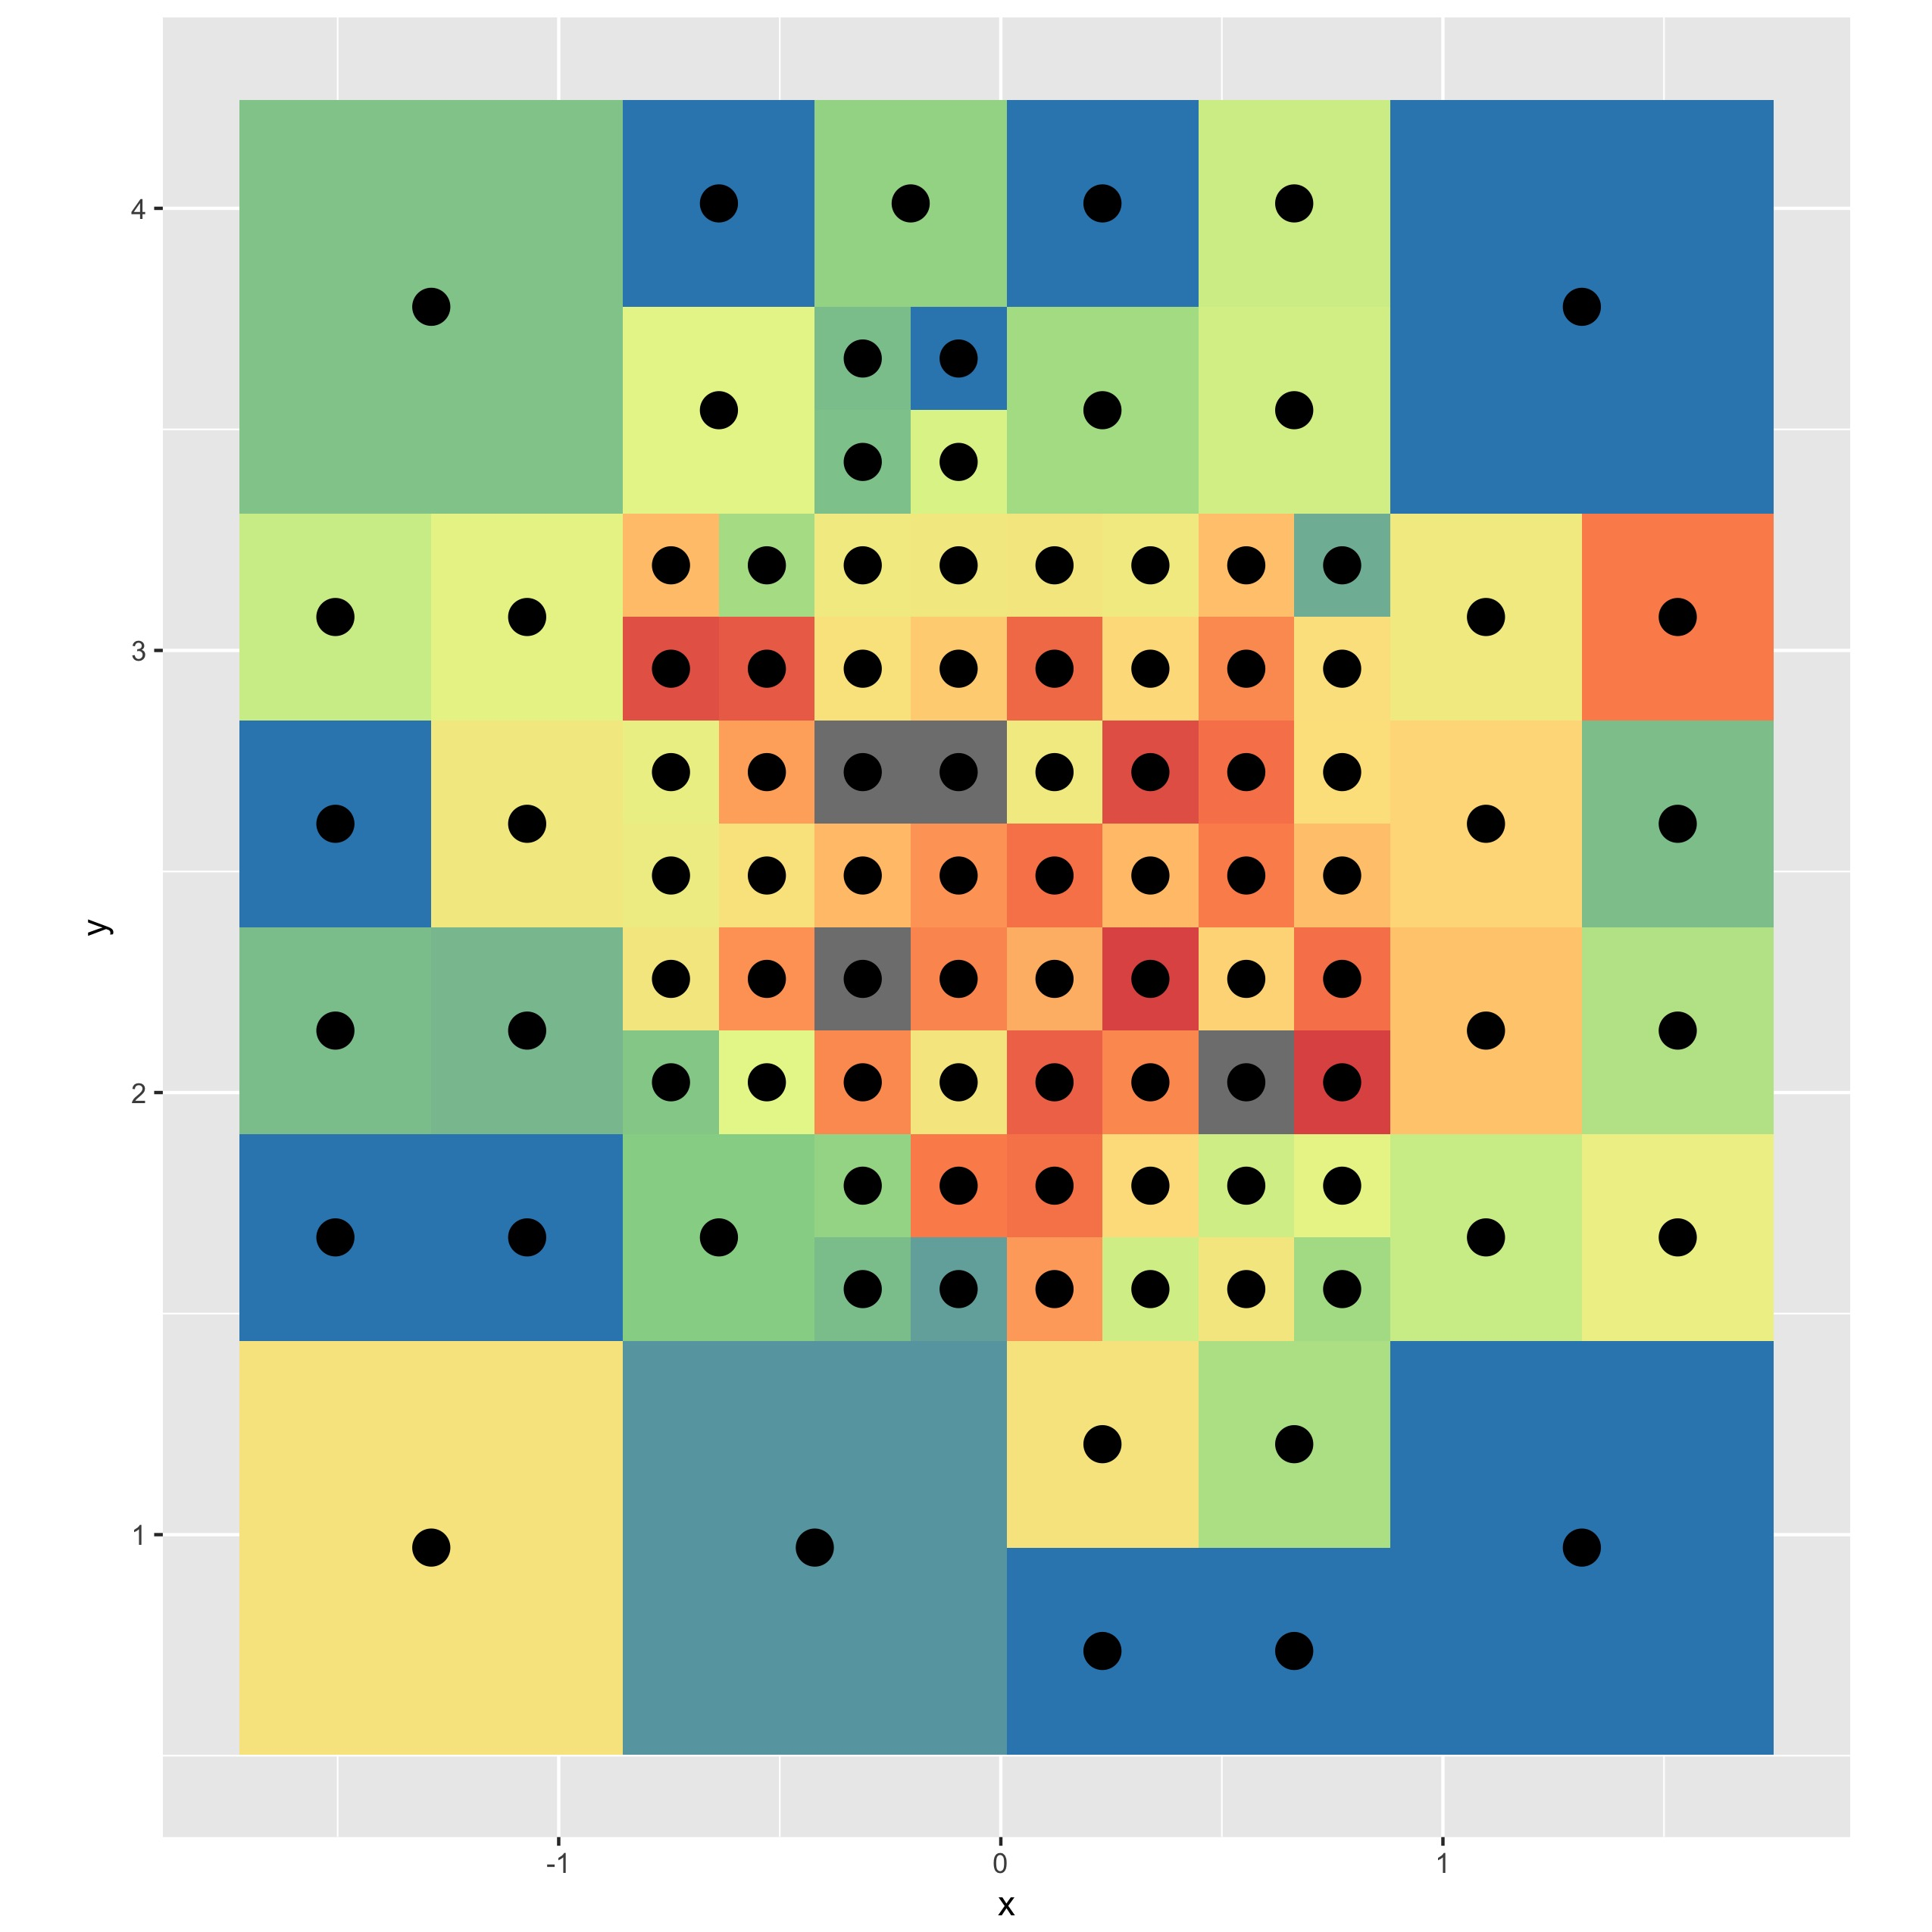
\includegraphics[scale=.08]{Images/knots.jpg}
	\caption{This map shows 97 PPM knots as variable-resolution heat map box centers. This Jhonny Peralta map used stopping rule $n_{b} < 200$.}
	\end{figure}
Using these 97 knots, for n = 300 observations, the PPM model fit generated 10,000 samples in three minutes. For n = 500 observation, 10,000 posterior draws required 4 minutes. For the same number of knots, but n = 1000 observations, 10,000 posterior draws required approximately seven minutes; and 37,500 draws required 23 minutes. The follow graphic shows VR empirical, GLM, and PPM fits for the same random n = 1000 subsample.
  \begin{figure}[H]
	\centering 
	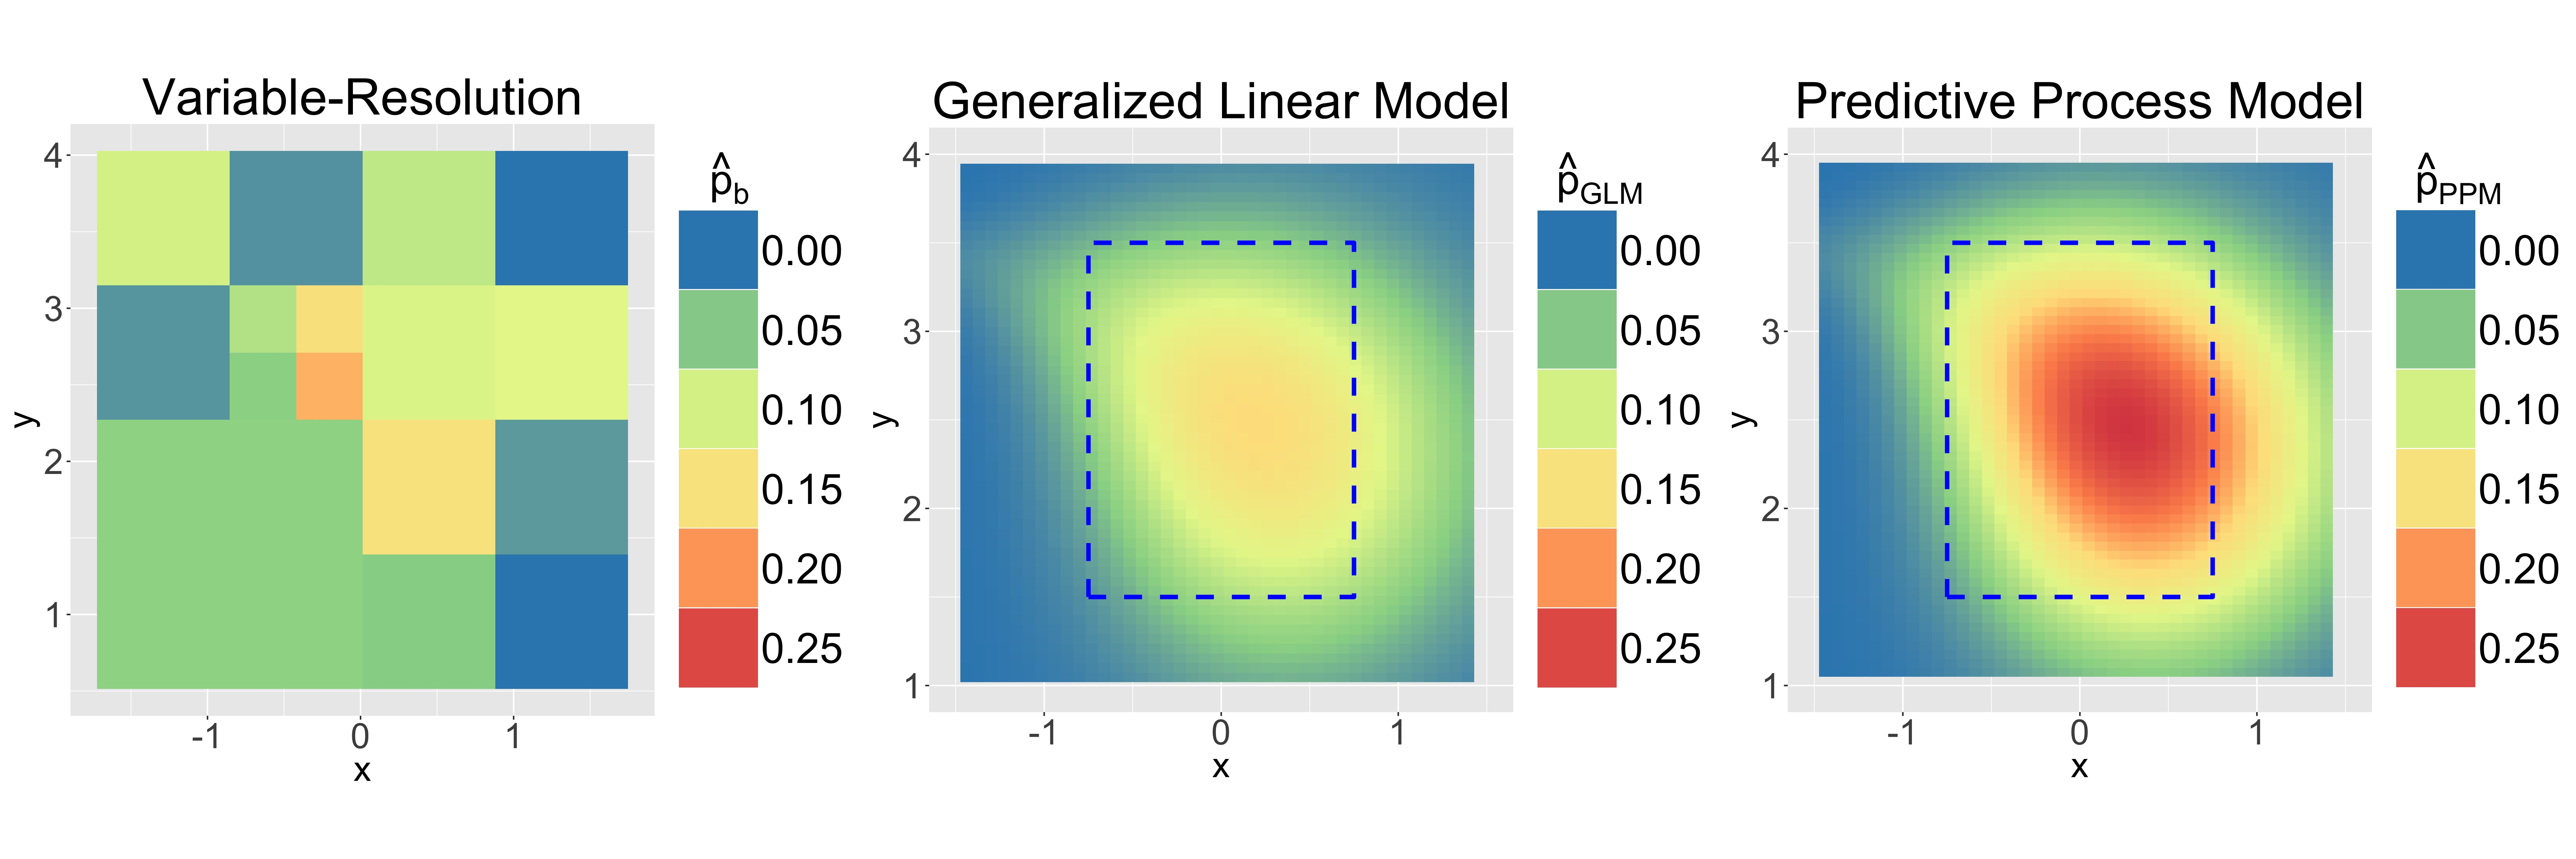
\includegraphics[scale=.05]{Images/VR_GLM_PPM.jpg}
	\caption{Empirical, generalized linear model, and predictive process model (97 knots) fits for a random subset of 1000 Jhonny Peralta observations. The predictive process model fit took approximately 23 minutes, while the generalized linear model fit took less than 10 seconds.}
	\label{fig:comps1}
	\end{figure}
Each fit tells its own story, with some overlap. All three maps appear to agree on Peralta's region of maximum success probabilities, but differ on the maximum. In particular, the GLM fit predicts much lower success probabilities than the PPM fit; even though they both assign similar shapes to the so called hot zone. The range of $\hat{p}$ on the empirical map more closely matches the GLM fit than the PPM fit. However, these observations only hold value as an interpretable example; the subset of n = 1000 observations falls far short of the available Peralta data.

Changing the number of knots to 49, but still using n = 1000 observations, the fit generated 30,000 posterior draws in seven minutes. Finally, for n = 3000 observations, still with 49 knots, the fit generated 37,500 posterior draws in 27 minutes. Notice that the elapsed time increased by only four minutes, despite going from n = 1000 to n = 3000 observations. This small increase results from reducing the number of knots from 97 to 49. These two factors---the number of observations and the number of knots---interactively influence the computational costs. Figure \ref{fig:comps2} below shows heap maps for the n = 3000 observation subset model fits. 
  \begin{figure}[H]
	\centering 
	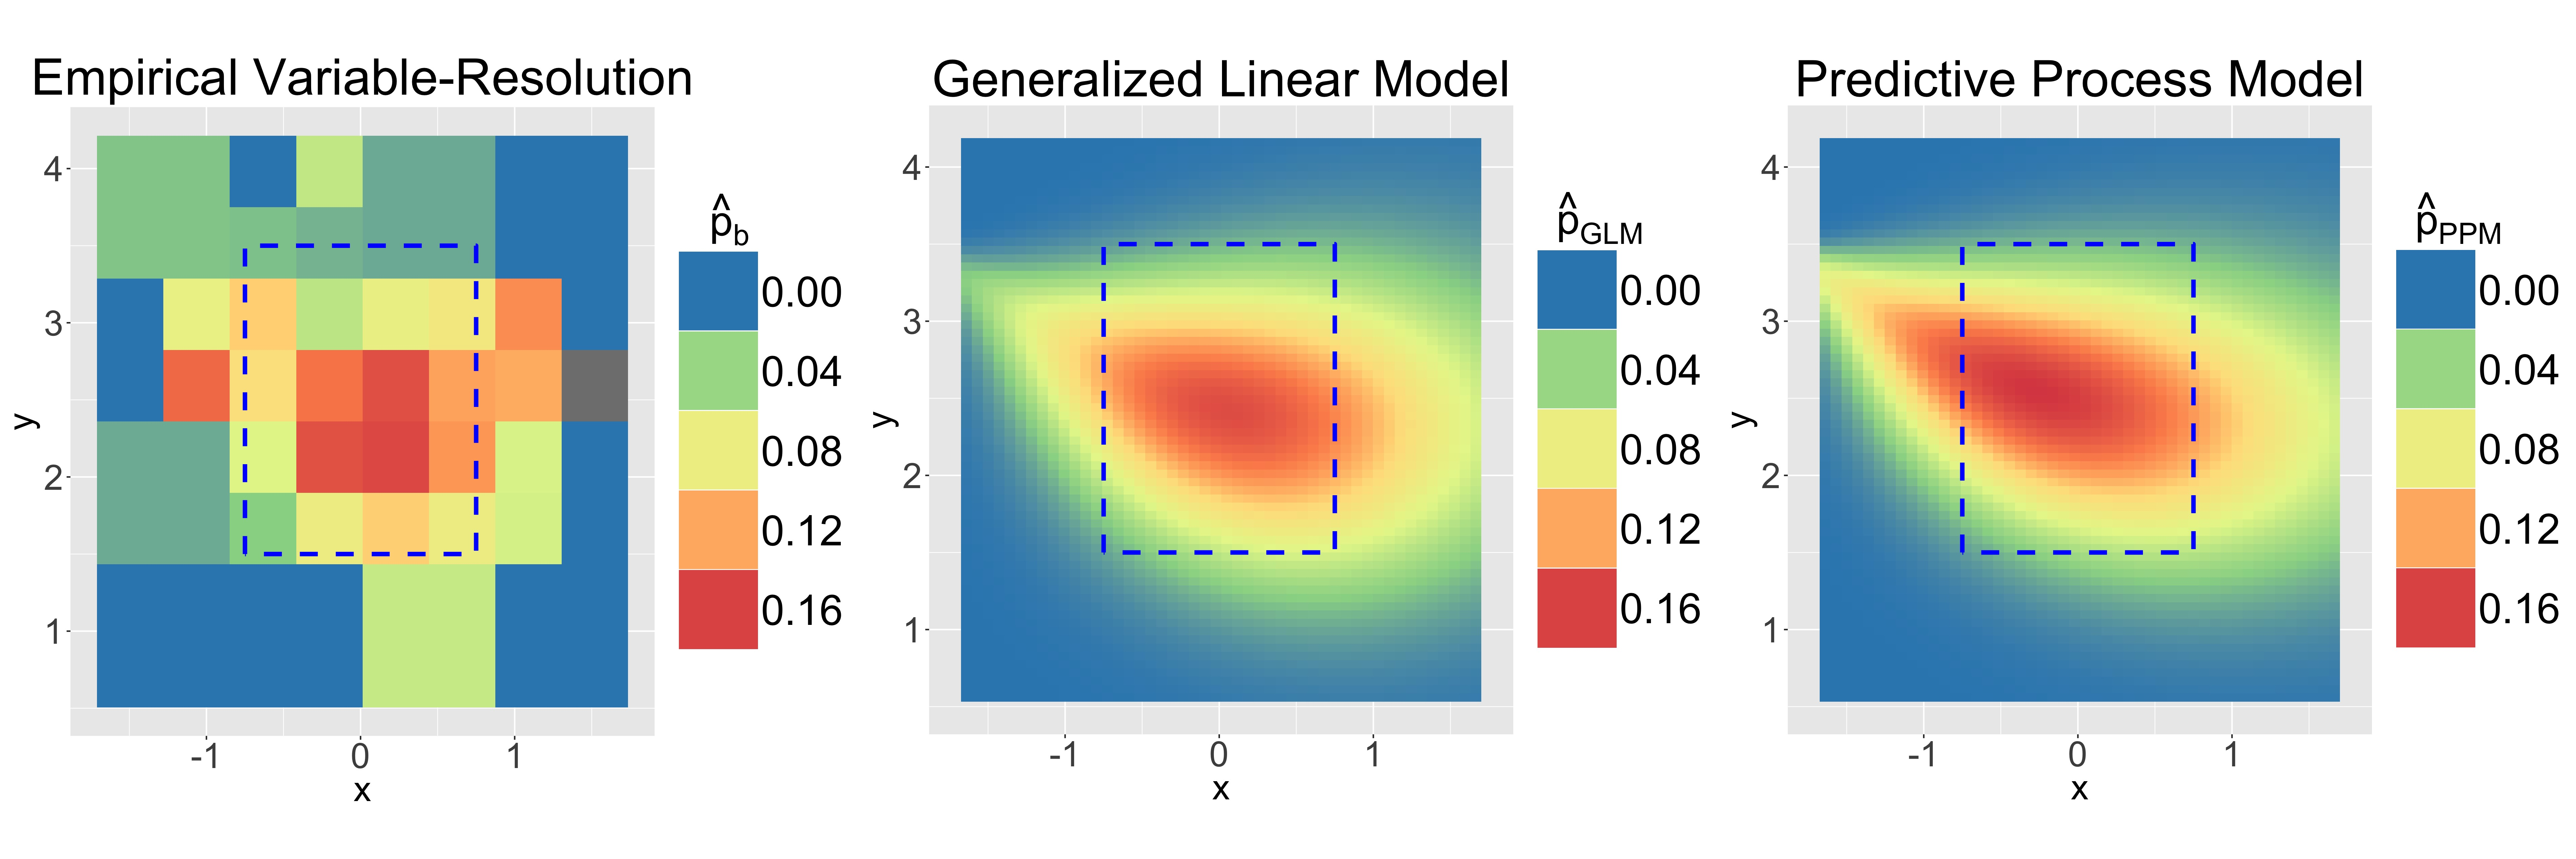
\includegraphics[scale=.05]{Images/VR_GLM_PPM_3000.jpg}
	\caption{Empirical, generalized linear model, and predictive process model (49 knots) fits for a random subset of 3000 Jhonny Peralta observations. The predictive process model fit took approximately 27 minutes, while the GLM fit took under 10 seconds.}
	\label{fig:comps2}
	\end{figure}
These maps show less variation than those in Figure \ref{fig:comps1}, probably owing to a larger set of observations. However, as before, this example serves only to demonstrate the tremendous increase in computational cost over the GLM model fit; and the tremendous increase in speed over model fitting in Stan, where we were unable to fit a model to an n = 3000 observation data set. 

\subsection{Discussion}
These results show promise in terms of speed. However, recall the Peralta data set contained 9,172 observations, and the final PPM fit described used only n = 3000 observations. Increasing the number of observations beyond 3000 slowed computations significantly, and closer to 9000 observations R sessions stalled and sometimes aborted. We seek a SGLMM fit to all 9,172 observations for comparison to the GLM fit, in order to answer: does a spatial random effect enhance the model sufficiently to justify its inclusion, given the increased computational demands?  

In the long run we seek a practical model, efficient enough to quickly re-fit with new data in real-time, on a personal computer. Ideally, such a model includes more covariates and categories; recall the numerous aspects of the hitter vs. pitcher contest we omitted. With these goals in mind, next we explore a sophisticated approximation technique that should reduce computation time even further.

\section{Integrated Nested Laplace Approximations} \label{INLA} % =================

Rue2009

Integrated Nested Laplace Approximation (INLA) works well for parameter estimation in Bayesian hierarchical models with latent Gaussian {\it Markov} random fields (GMRFs), but not directly with GRFs \citep{Rue2007}.

Adding a specific neighborhood structure to a GRF yields a GMRF \citep{Rue2007}. The neighborhood structure explicitly defines when random effects at two locations are neighbors, and the Markov structure assigns non-zero correlation to two random effects if and only if the two effects are neighbors. 

The importance of the distinction between GRFs and GMRFs lies in the sparse precision matrix of a GMRF, because INLA's speedy computations rely on sparse precision matrices. Therefore, we need to represent our continuous GRF as a discrete GMRF in order to use INLA; stochastic calculus provides a link. Namely, the stochastic partial derivative of a {\it Matern} GRF equals a Gaussian random field white noise process \citep{Lindgren2011}. This stochastic partial differential equation (SPDE) buttresses a method to approximate a {\it Matern} GRF with a GMRF, in the form of a piecewise linear basis representation. The approach, known as Finite Element Method (FEM), projects the SPDE onto a basis representation \citep{Dhatt2012}, consisting of deterministic basis functions, defined by a triangulation of the domain, and GMRF weights. This discrete basis representation, with a sparse precision matrix, qualifies for INLA. In the next section we formally define a GMRF.


\subsection{Gaussian Markov Random Fields}

To formally define a GMRF \citep{Rue2007}, let $\pmb{x} = \{ x_{i}:i \in \mathscr{V} \}$, where $\mathscr{V} = \{1,\dots,n\}$, for $n = |\mathscr{V}|$-dimensional Gaussian random vector $\pmb{x}$. Now define graph $\mathscr{G} = \{ \mathscr{V}, \mathscr{E} \}$, containing vertices $\mathscr{V}$ and edges $\mathscr{E}$. Vertices $x_{i}$ and $x_{j}$ are conditionally independent given all other elements of $\pmb{x}$, if and only if $\{i, j\} \notin \mathscr{E}$. The neighborhood structure defined by this graph yields GMRF $\pmb{x}$ with respect to $\mathscr{G}$, where $i \sim j$ denotes $i$ neighbors $j$. The edges in $\mathscr{E}$ correspond exactly to the non-zero elements of the GMRF precision matrix $\pmb{Q}$; $\{ i, j \} \in \mathscr{E}$ if and only if $Q_{ij} \neq 0 \text{ for } i \neq j$. Non-zero elements of $Q_{ij}$ correspond to neighbors.

Integrated Nested Laplace Approximations (INLAs) require a GMRF structure for the latent random effect. However, our original model contains a GRF. Therefore, we use a stochastic partial differential equations (SPDEs) as an explicit link between GRFs and GMRFs. Section \ref{SPDE} describes the SPDE link. 

\subsection{Stochastic Partial Differential Equation (SPDE)} \label{SPDE}

\cite{Whittle1954} declared $\text{Matern}_{\nu = 1}$ spatial correlation structure---not the exponential ($\text{Matern}_{\nu = 1/2}$)---the ``elementary correlation'' function in two dimensions. The following defines the Matern family of covariance functions.
$$\text{C}(h) = \frac{\sigma^{2}}{2^{\nu - 1}\Gamma(\nu)}(\kappa h)^{\nu}K_{\nu}(\kappa h)$$
This parameterization includes range parameter $\kappa > 0$, smoothness parameter $\nu > 0$, scale parameter $\sigma^{2}$, and modified Bessel function $K_{\nu}(\cdot)$ \citep{Schabenberger2004}. Matern random fields solve the following SPDE \citep{Whittle1954},
\begin{equation} \label{eq:spde1}
(\kappa^{2} - \Delta)^{\alpha/2}x(\pmb{s}) = \mathcal{W}(\pmb{s}),
\end{equation}
which includes the Laplace operator $\Delta = \sum_{i=1}^{d} \frac{\partial^{2}}{\partial x_{i}^{2}}$; spatial scale (range) parameter $\kappa$; smoothness parameter $\alpha$; and Gaussian spatial white noise process $\mathcal{W}(\pmb{s})$. The SPDE and Matern coupling dictates $\alpha = \nu + d/2$, where d = 2 for $\mathbb{R}^{2}$; and $$\sigma^{2} = \frac{\Gamma(\nu)}{\Gamma(\alpha)(4\pi)^{d/2}\kappa^{2\nu}}.$$
Based on \citep{Whittle1954}, \citep{Mondal2017}, and \citep{Lindgren2015}, we use $\nu = 1$, which implies $\alpha = 2$. This specification simplifies the SPDE to 
\begin{equation} \label{eq:spde}
(\kappa^{2} - \Delta)x(\pmb{s}) = \mathcal{W}(\pmb{s});
\end{equation}
the Matern covariance to 
\begin{equation} \label{eq:matern}
\text{C}(h) = \sigma^{2}(\kappa h)K_{1}(\kappa h);
\end{equation}
and the variance to $\sigma^{2} = \frac{1}{4 \pi \kappa}$.

Recall equation \ref{eq:SGLMM}; until now we assumed an exponential covariance structure for $w(\pmb{s}_{ij})$. This section marks a shift: based on \citep{Whittle1954}, \citep{Mondal2017}, and \citep{Lindgren2015}, now we assume a $\text{Matern}_{\nu = 1}$ covariance structure for random effect $w(\pmb{s}_{ij})$. 

The next three subsections organize and delineate the steps to use the SPDE in equation \ref{eq:spde} to map a $\text{Matern}_{\nu = 1}$ GRF to a GMRF, and thus allow us to use the INLA procedure \citep{Lindgren2011}.

\subsubsection{Piecewise Linear Basis Representation}
The Finite Element Method, projects the SPDE onto a piecewise linear basis representation \citep{Simpson2012}. The basis representation,
\begin{equation} \label{eq:basisrep}
x(\pmb{s}) = \sum_{k=1}^{n} \psi_{k}(\pmb{s})x_{k},
\end{equation}
contains deterministic basis functions, $\psi_{k}(\cdot)$; and GMRF weights $\pmb{x} = \{x_{1},\dots,x_{n}\}$. The two combine in \ref{eq:basisrep} so that the distribution of $x(\pmb{s})$ approximates the Matern GRF that solves the SPDE, but retains a sparse precision matrix and its accordant computational advantages. 

The next section describes how the SPDE link produces the the deterministic basis functions in equation \ref{eq:basisrep}.

\subsubsection{Deterministic Basis Function}

A triangulation of the domain defines the deterministic component, $\psi_{k}(\pmb{s})$, of the basis representation in equation \ref{eq:basisrep}. Figure \ref{fig:basis} illustrates how domain triangulation determines a basis function \citep{Simpson2012}.
  \begin{figure}[H]
	\centering 
	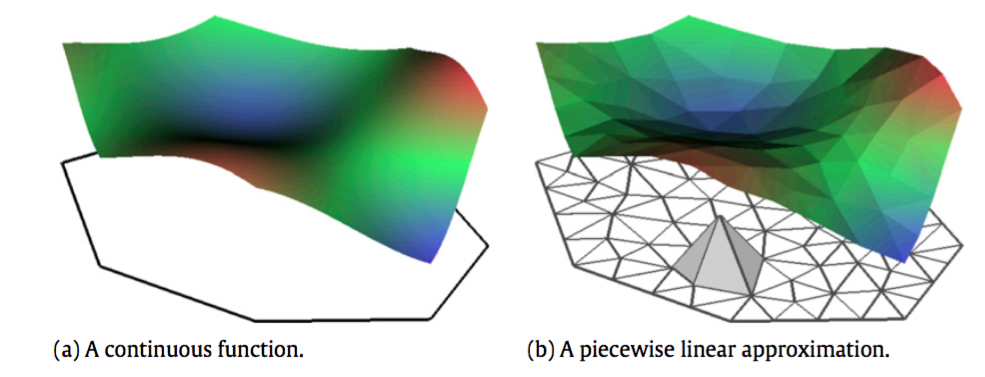
\includegraphics[scale=.4]{Images/PLBF.jpg}
	\caption{A Gaussian Markov random field, defined as the piecewise linear basis function $  x(\pmb{s}) = \sum_{k=1}^{n} \protect\psi_{k}(\pmb{s})x_{k}$, approximates a Matern GRF. This image illustrates how a triangular mesh over the domain determines basis functions $\protect\psi_{k}(\pmb{s})$ 
	\citep{Simpson2012}.}
	\label{fig:basis}
	\end{figure}
Keep in mind that a realization of a GRF essentially constitutes a function, and Figure \ref{fig:basis} shows how a discrete piecewise linear basis function approximates a continuous function \citep{Simpson2012}. Notice, $\psi_{k}(\pmb{s}) = 1$ at the $k\text{th}$ vertex, $0$ at all other vertices, and surface function values for triangle interior points are linear combinations of the three home triangle vertices.
 
The next section describes how the SPDE link produces the GMRF weights in the basis function (equation \ref{eq:basisrep}).

\subsubsection{GMRF Weights}

Stochastic calculus identities provide a way to calculate the weights in the basis representation of \ref{eq:basisrep}. To start, let $$\langle f, g \rangle = \int f(\pmb{u}) g(\pmb{u}) d\pmb{u}.$$ 
Then we find weights $\pmb{x}$ such that, for a set of test functions $\phi_{k}$, the following equality holds \citep{Lindgren2011}:
\begin{equation} \label{eq:stoch}
\left[ \left< \phi_{k}, (\kappa^{2} - \Delta)^{\alpha/2} \pmb{x} \right> \right]_{k = 1, \hdots, n} \overset{D}{=} \Big[ \langle \phi_{k}, \mathcal{W} \rangle \Big]_{k = 1, \hdots, n}.
\end{equation}

The solution, weight vector $\pmb{x}$, gives the stochastic weak solution solution to the SPDE in equations \ref{eq:spde1} and \ref{eq:spde}. \citep{Mao2007}, \cite{Lindstrom2014}. Following \cite{Lindgren2011}, we use the Galerkin solution where $\alpha = 2$ and $\phi_{i} = \psi_{i}$. Therefore, replace $\pmb{x}$ in equation \ref{eq:stoch} with basis function representation $\Sigma_{k}\psi_{k}w_{k}$:
$$ \left[ \left< \phi_{i}, (\kappa^{2} - \Delta)^{\alpha/2} \psi_{j} \right> \right]_{i,j}\pmb{w} \overset{D}{=} \Big[ \langle \phi_{k}, \mathcal{W} \rangle \Big]_{k}.$$
Next, let $\alpha = 2$ and $\phi_{i} = \psi_{i}$ as in the Galerkin solution, and simplify to get:
$$ \Big(
\kappa^{2} [ \langle \psi_{i}, \psi_{j} \rangle ] + [ \langle \psi_{i}, -\Delta \psi_{j} \rangle ]
\Big) \pmb{w} \overset{D}{=} \Big[ \langle \psi_{k}, \mathcal{W} \rangle \Big]. $$

Simplify notation by letting $\pmb{C}_{i,j} = \langle \psi_{i}, \psi_{j} \rangle$, and $ \pmb{G}_{i,j} = \langle \psi_{i}, - \Delta \psi_{j} \rangle$, so that
$$ \left(
\kappa^{2} \pmb{C} + \pmb{G} \right) \pmb{w} \overset{D}{=} \text{N}(\pmb{0},\pmb{C}).$$
Thus, $\pmb{w} \sim \text{N}(\pmb{0}, \pmb{Q}^{-1})$, where:
\begin{equation} \label{eq:Q}
\pmb{Q}_{\kappa} = \left( \kappa^{2} \pmb{C} + \pmb{G} \right)^{T} \pmb{C}^{-1} \left( \kappa^{2} \pmb{C} + \pmb{G} \right).
\end{equation}
% However, $\pmb{C}^{-1}$ has a sparse precision matrix, so replace $\pmb{C}$ in equation \ref{eq:Q} with diagonal matrix $\widetilde{\pmb{C}}$:
% $$ \widetilde{\pmb{C}}_{i,i} = \langle \psi_{i}, \pmb{1} \rangle = \int \psi_{i}(\pmb{s}) d\pmb{s}.$$ 
% \begin{equation} \label{eq:Q2}
% \pmb{Q}_{\kappa} = \left( \kappa^{2} \widetilde{\pmb{C}} + \pmb{G} \right)^{T} \pmb{C}^{-1} \left( \kappa^{2} \widetilde{\pmb{C}} + \pmb{G} \right).
% \end{equation}
Note that this solution specifies the distribution of the weights $x_{k}$ in the basis representation of equation \ref{eq:basisrep}, not $x(\pmb{s})$ itself.

With this representation achieved, via the SPDE link, we move on to INLA, which approximates the model parameters.

\subsection{Integrated Nested Laplace Approximations (INLA)}

INLA estimates the marginal posterior distributions for latent field parameters, $p(x_{i}|\pmb{y})$; and covariance hyperparameter posterior $p(\theta|\pmb{y})$. This means INLA does not estimate posteriors $p(\pmb{x}|\pmb{y})$ and $p(\pmb{x},\pmb{\theta}|\pmb{y})$. We break the INLA procedure into three steps to facilitate explanation; their details comprise the next three subsections.

\subsubsection{Step 1, Gaussian Approximation} % ======= ======

INLA begins by ``matching the mode and curvature at the mode'' of Gaussian estimator $p_{G}(\pmb{x}|\pmb{\theta}, \pmb{y})$ to that of $p(\pmb{x}|\pmb{\theta}, \pmb{y})$ \citep{Rue2005}. Note that INLA requires Gaussian priors for all parameters, excluding covariance hyperparameters. INLA also requires conditional independence: $p(\pmb{y}|\pmb{x}, \pmb{\theta}) = \prod_{i} p(y_{i}|\pmb{x}_{i},\pmb{\theta})$. Our analysis satisfies this requirement, and therefore $$p(\pmb{x}|\pmb{\theta},\pmb{y}) \propto \text{exp}\left(-\frac{1}{2}\pmb{x}^{T}\pmb{Q x} + \sum_{i} \text{log }p(y_{i}|\pmb{x}_{i},\pmb{\theta}) \right).$$ Assuming Gaussian priors and conditional independence, the INLA Gaussian approximation for $p(\pmb{x}|\pmb{\theta}, \pmb{y})$ takes the form
\begin{equation} \label{eq:ga}
p_{G}(\pmb{x}|\pmb{\theta},\pmb{y}) \propto \text{exp} \left( -\frac{1}{2}(\pmb{x-\mu})^{T} (\pmb{Q} + \text{diag}(\pmb{c}) ) (\pmb{x - \mu}) \right),
\end{equation}
where vectors $\pmb{c}$ and $\pmb{\mu}$ depend on second order Taylor expansions of $f(\pmb{x}) = \sum_{i} \text{log }p(y_{i}|\pmb{x}_{i},\pmb{\theta})$ about the mode \citep{Lindstrom2014}. A Newton-Raphson algorithm iteratively computes the mode and precision matrix until convergence \citep{Rue2009}. Step 2 uses the approximation in \ref{eq:ga} to approximate $p(\pmb{\theta}|\pmb{y})$.

\subsubsection{Step 2, Laplace Approximation}  % ====== ======

This step begins with two sides of a familiar identity, and its subsequent rearrangement.
\begin{align}
p(\pmb{y} , \pmb{x} | \pmb{\theta}) = p(\pmb{y} | \pmb{x}, \pmb{\theta}) p(\pmb{x} | \pmb{\theta})  &= p(\pmb{x} | \pmb{y}, \pmb{\theta}) p(\pmb{y} | \pmb{\theta}) \\
\frac{p(\pmb{y} | \pmb{x}, \pmb{\theta}) p(\pmb{x} | \pmb{\theta})} {p(\pmb{x} | \pmb{y}, \pmb{\theta})} &= p(\pmb{y} | \pmb{\theta})  
\end{align}
Next, substitute this last formulation of $p(\pmb{y}|\pmb{\theta})$ into the foundational Bayesian proportionality.
\begin{align}
p(\theta|\pmb{y}) & \propto p(\pmb{y}|\pmb{\theta})p(\pmb{\theta}) \\
& \propto \frac{p(\pmb{y} | \pmb{x}, \pmb{\theta}) p(\pmb{x} | \pmb{\theta})}{p(\pmb{x} | \pmb{y}, \pmb{\theta})} \cdot p(\pmb{\theta})
\end{align}
For a given $\pmb{\theta}$, let $\pmb{x}_{0} = \text{argmax}_{x}p(\pmb{x}|\pmb{y},\pmb{\theta})$. Then,
\begin{equation} \label{eq:la}
p(\pmb{\theta}|\pmb{y}) \approx \tilde{p}(\pmb{\theta}|\pmb{y}) \propto  \frac{p(\pmb{y} | \pmb{x}_{0}, \pmb{\theta}) p(\pmb{x}_{0} | \pmb{\theta})}{p_{G}(\pmb{x}_{0} | \pmb{y}, \pmb{\theta})} \cdot p(\pmb{\theta}),
\end{equation}
with the Taylor approximation of $f(\pmb{x}) = \sum_{i} \text{log }p(y_{i}|x_{i})$ in $p_{G}(\pmb{x} | \pmb{y}, \pmb{\theta})$ expanded about $\pmb{x}_{0}$. Then, we have approximate maximum likelihood estimate $\hat{\pmb{\theta}}_{\text{ML}} \approx \text{argmax}_{\theta} \tilde{p}(\pmb{\theta}|\pmb{y})$. \cite{Tierney1986} showed this approximation matches the Laplace approximation. 

Next, in Step 3, we use the results of Step 1 and Step 2 to nest and numerically integrate the Laplace approximations to approximate marginal posteriors.

\subsubsection{Step 3, Numerical Integration} % === === === === ===
Using the Gaussian approximation, $p_{\text{G}}(x_{j}|\pmb{\theta, y})$, from equation \ref{eq:ga} in Step 1; and the Laplace approximation, $\tilde{p}(\pmb{\theta}|\pmb{y})$, from equation \ref{eq:la} in Step 2; we can now integrate numerically to find posterior marginals $p(x_{i}|\pmb{y})$ and $p(\theta_{i}|\pmb{y})$. 
        $$ p(x_{j} | \pmb{y}) \approx \int p_{\text{G}}(x_{j}|\pmb{\theta, y})\tilde{p}(\pmb{\theta}|\pmb{y}) d\pmb{\theta} $$
        $$ p(\theta_{k} | \pmb{y}) \approx \int \tilde{p}(\pmb{\theta}|\pmb{y}) d\pmb{\theta}_{-k} $$
        
For additional details of the procedure, see \cite{Rue2009}. We implement the SPDE-INLA procedure of the previous two subsections with the R package \verb|INLA| \citep{INLA}, \citep{Lindgren2015}.
        
\subsection{Results}
We fit our SGLMM with the same n = 1000 and n = 3000 observations used for the PPM fits in Section \ref{PPMresults}, and shown in Figures \ref{fig:comps1} and \ref{fig:comps2}. The INLA model fit with n = 1000 observations required approximately 5 seconds; and the n = 3000 fit required approximately 9 seconds. Most impressively, the INLA fit to all 9172 Peralta observations required approximately 34 seconds. This marks the first complete fit of our SGLMM to all Peralta observations, in our research. Figure \ref{fig:INLA} shows all three INLA model fits.
  \begin{figure}[H]
	\centering 
	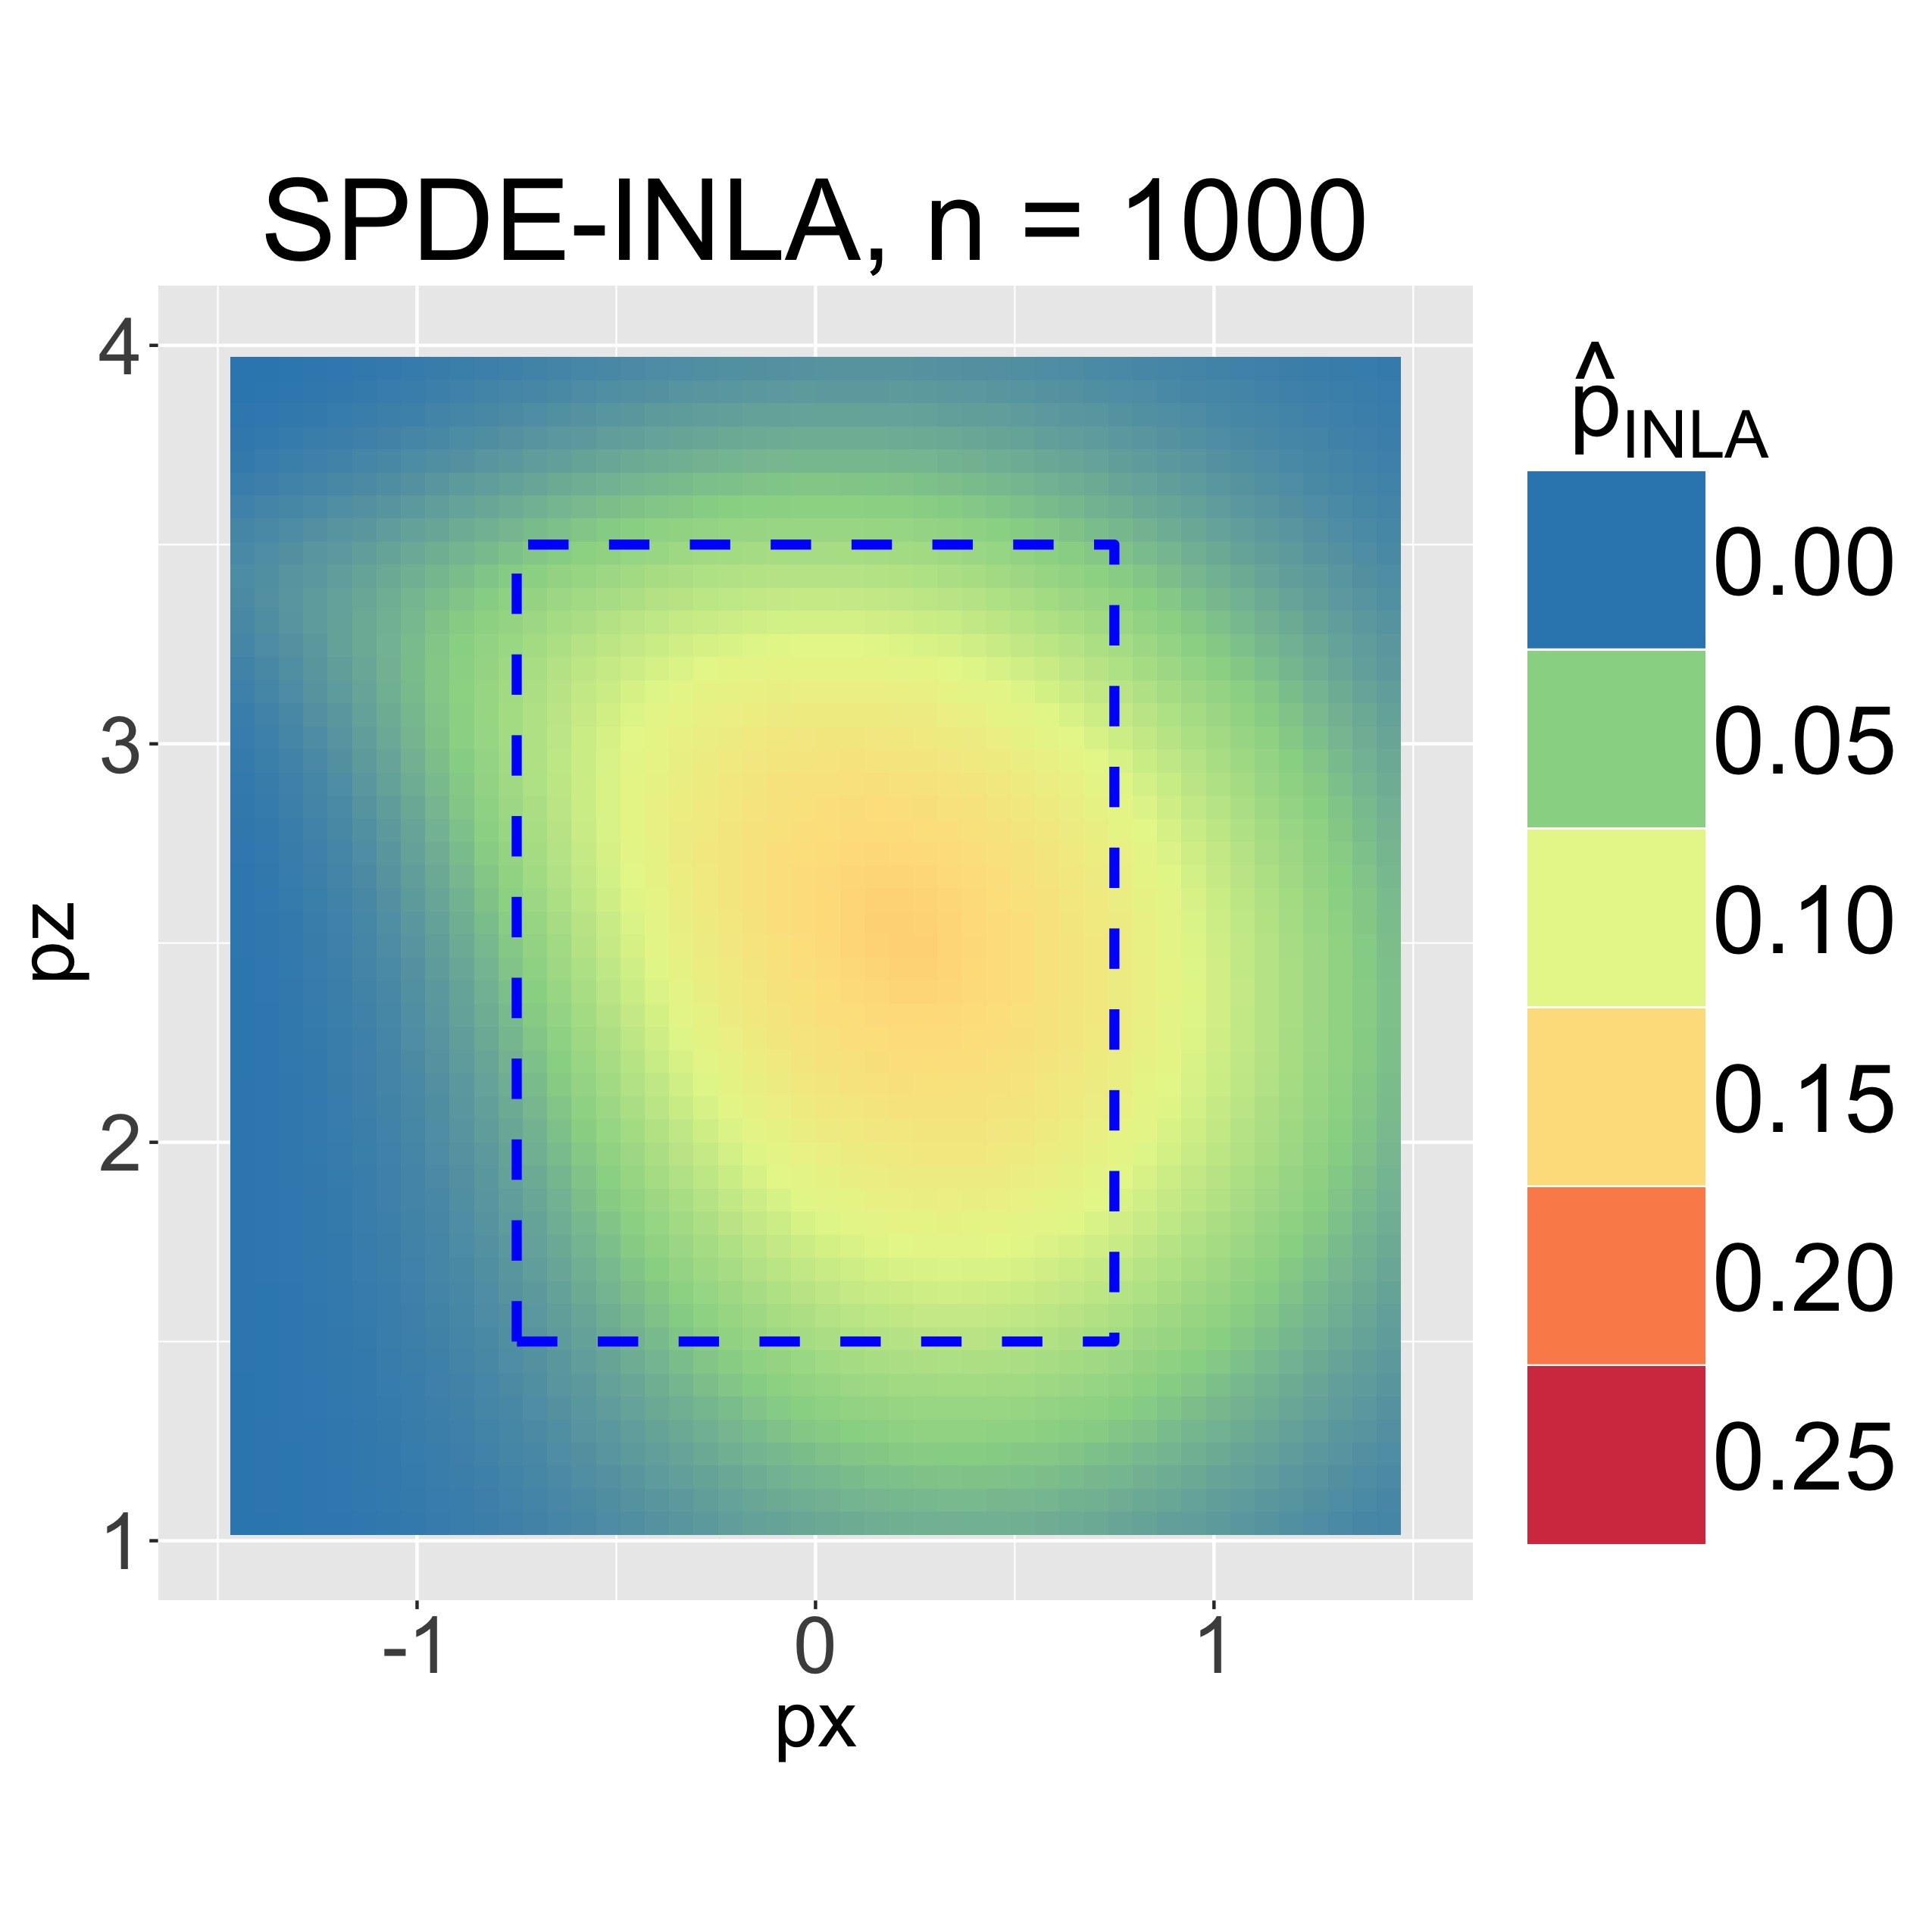
\includegraphics[scale=.05]{Images/INLA1000.jpg}	
	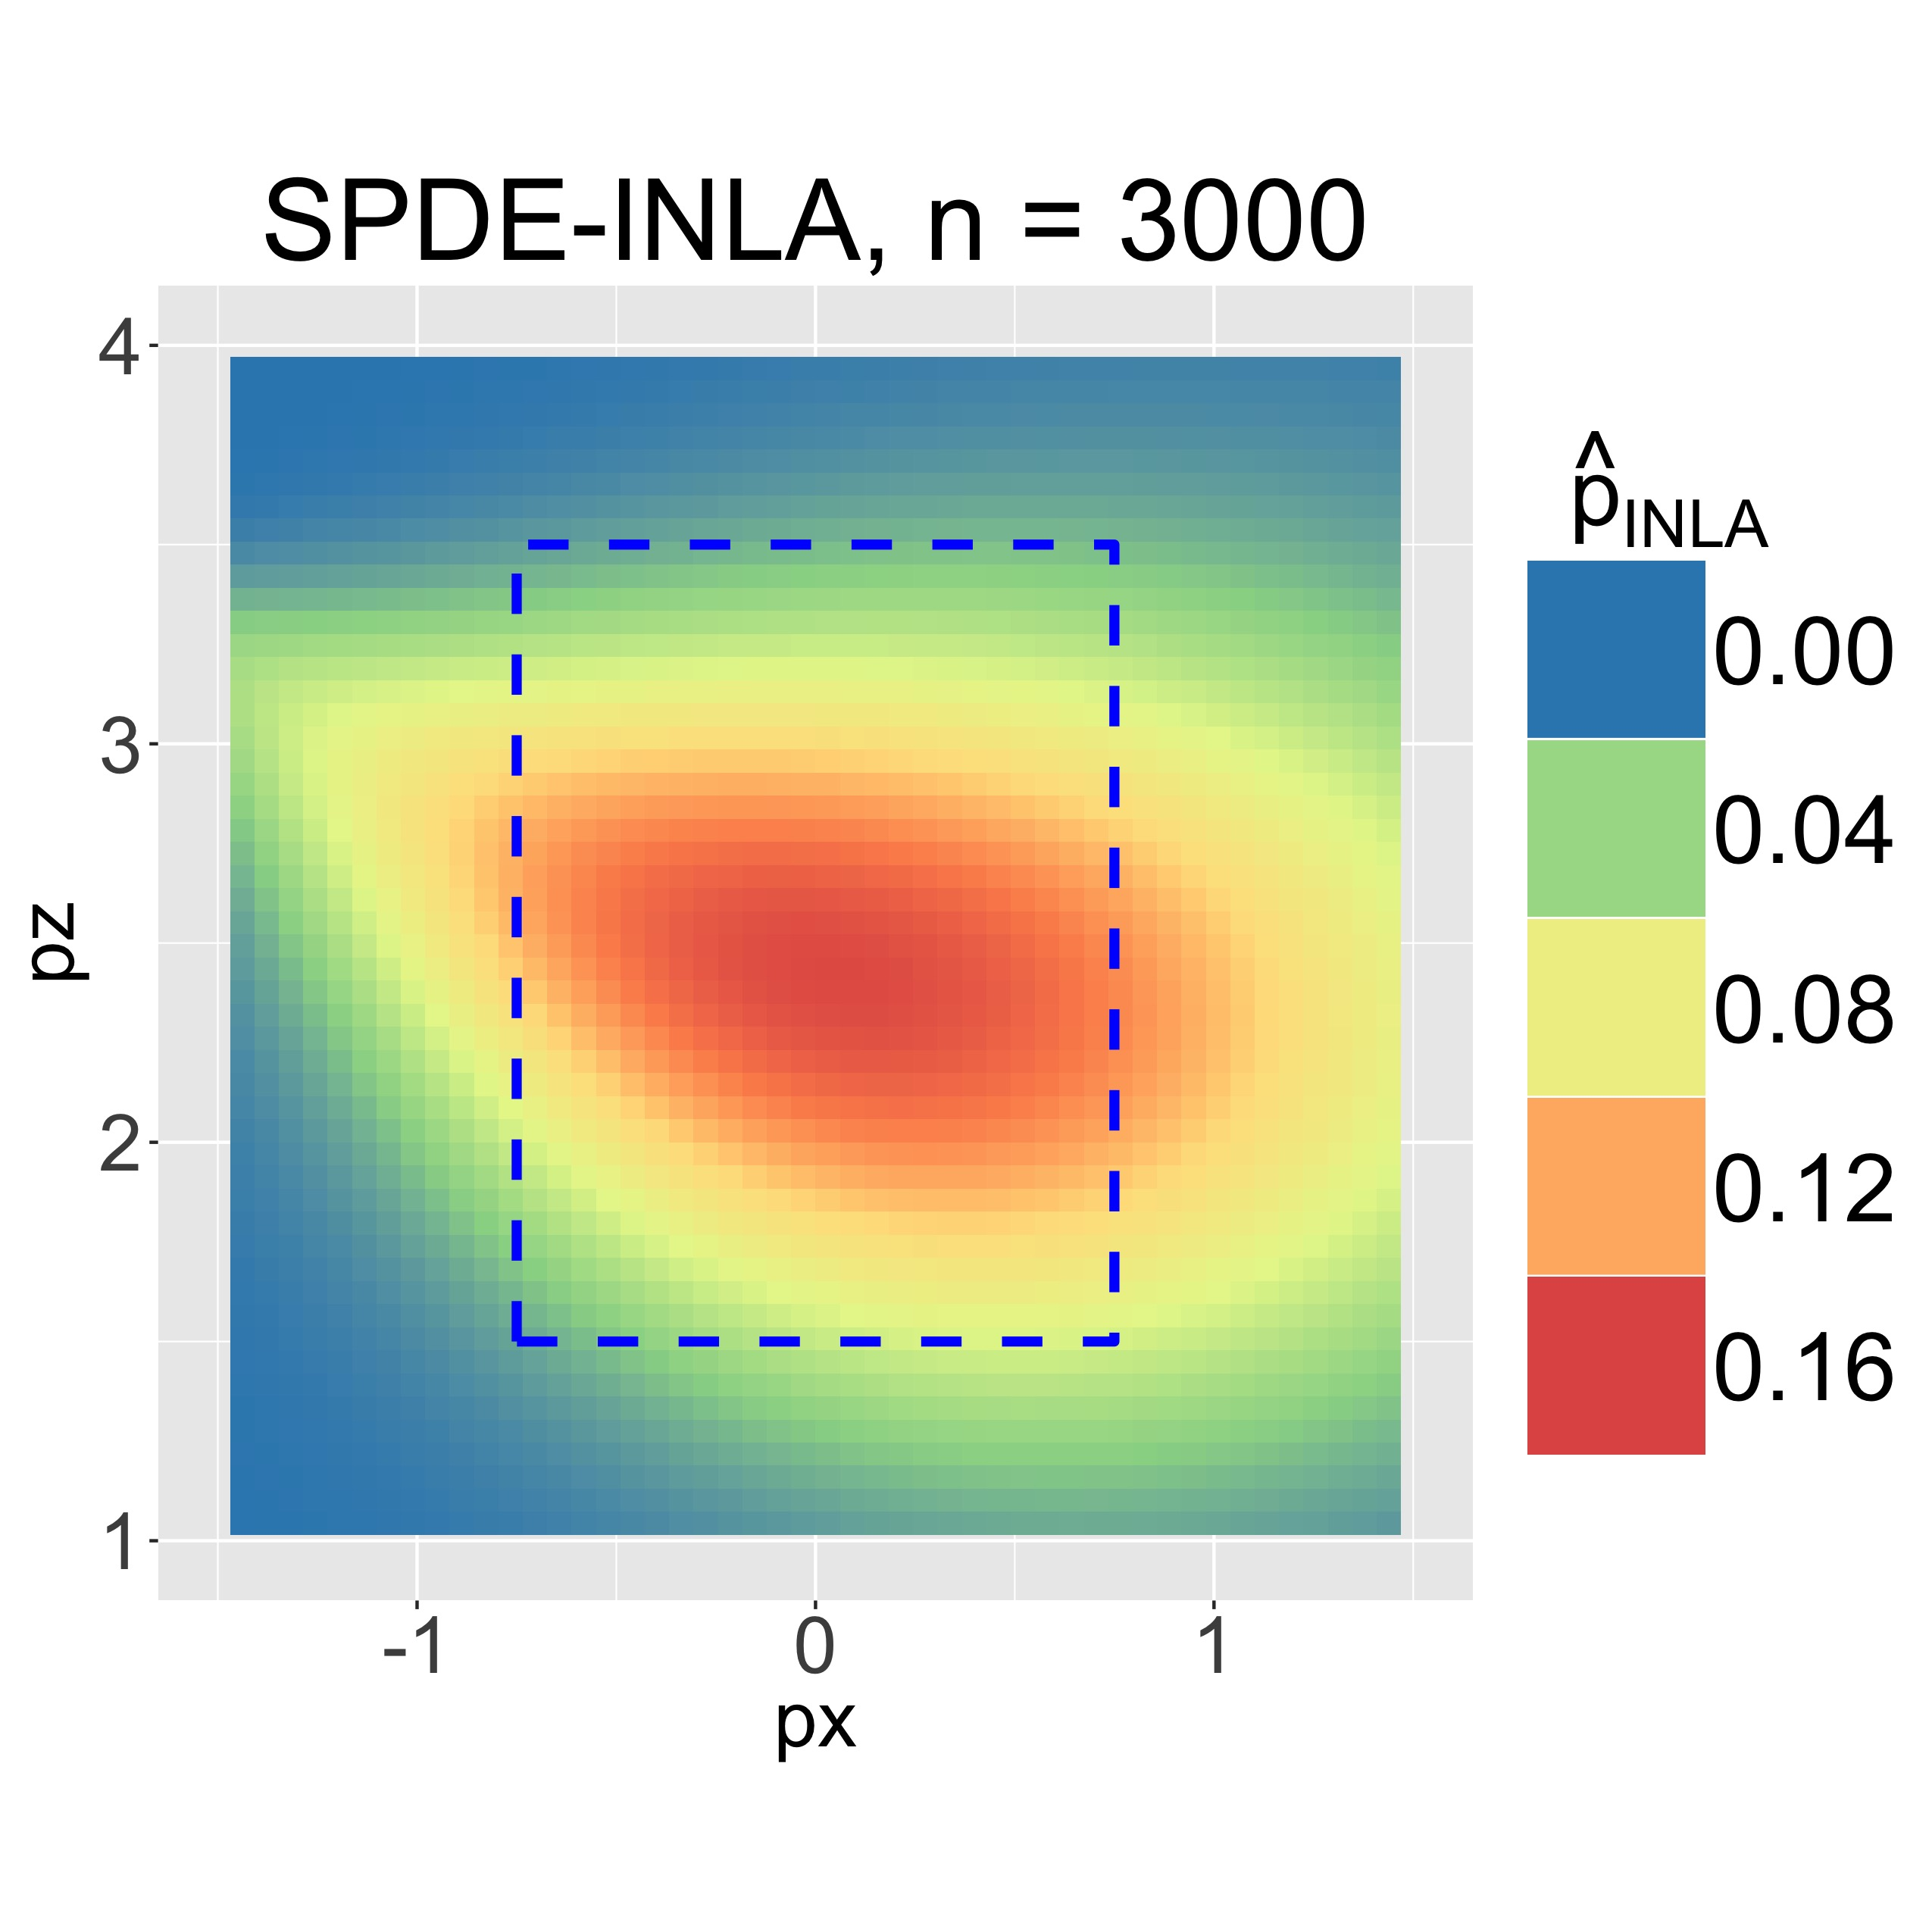
\includegraphics[scale=.05]{Images/INLA3000.jpg}
	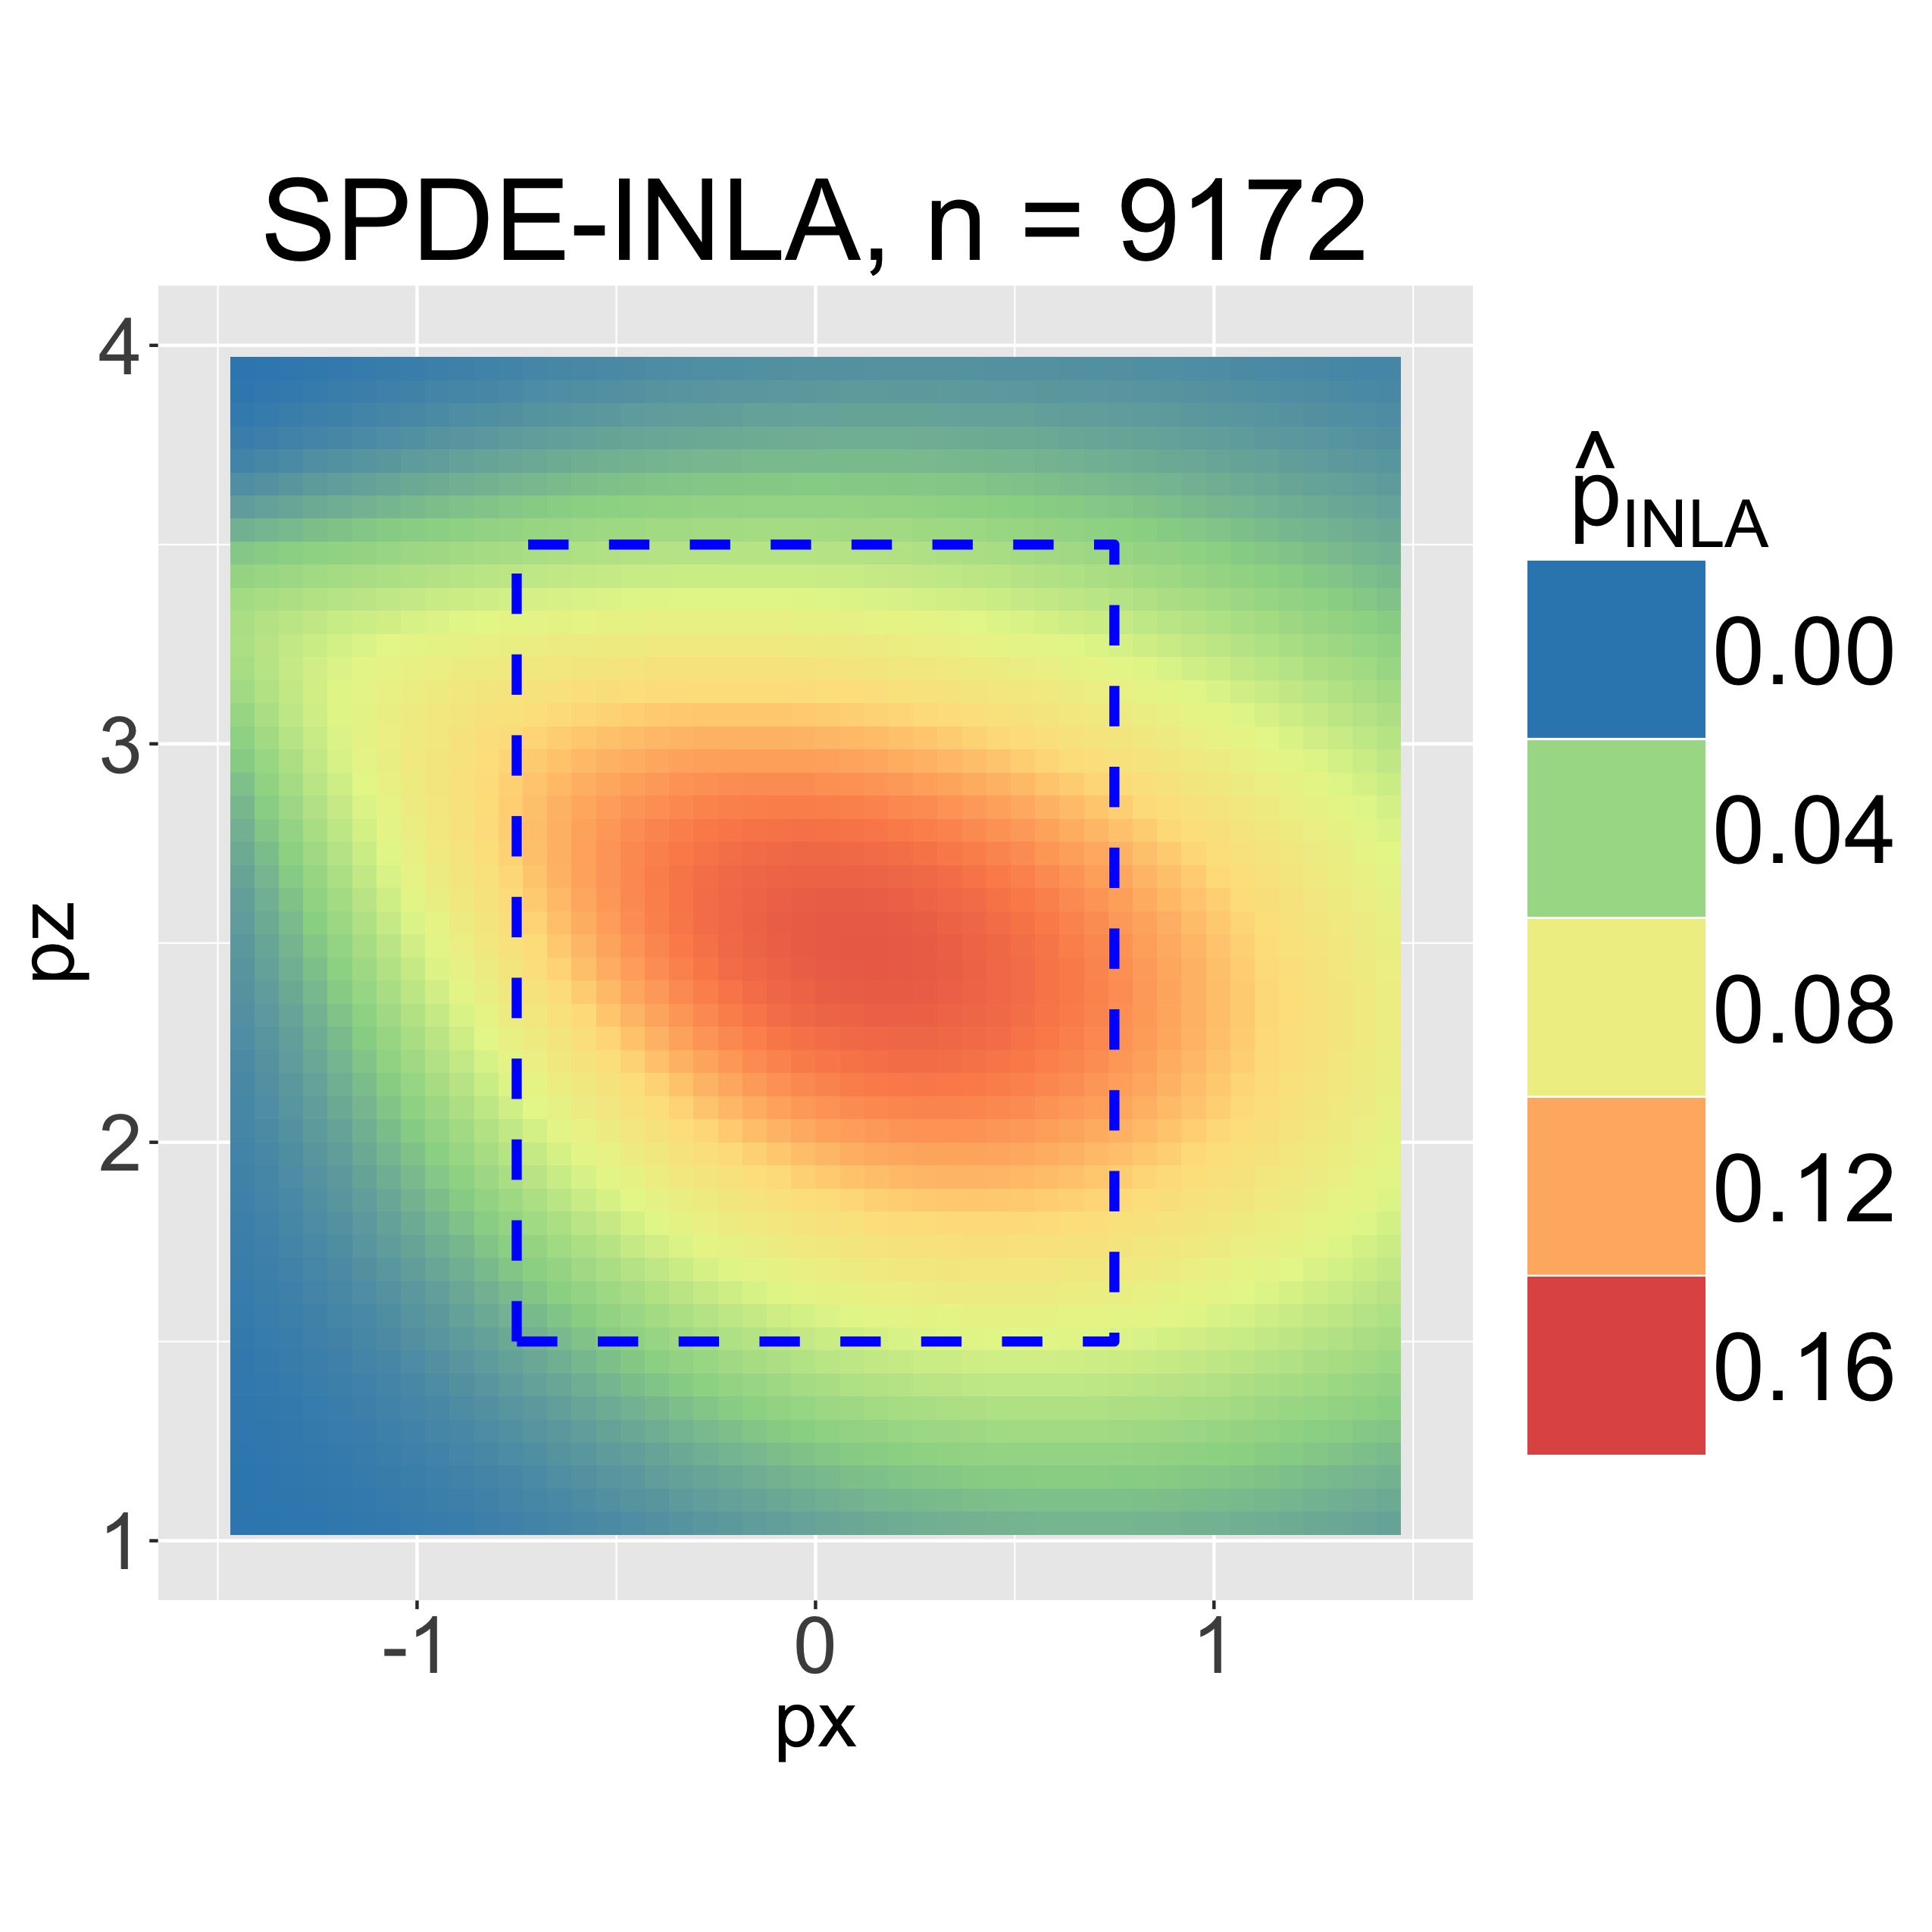
\includegraphics[scale=.05]{Images/INLA9172.jpg}
	\caption{Integrated nested Laplace approximation model fits. The model fit for n = 1000 observations required approximately five seconds; compare this fit to Figure \ref{fig:comps1}. The n = 3000 model fit required approximately nine seconds; compare this map to Figure \ref{fig:comps2}. Finally, the INLA fit with all n = 9172 Peralta observations required approximately 34 seconds; compare this map to the variable-resolution empirical heat map in Figure \ref{fig:interp}.}
	\label{fig:INLA}
	\end{figure}
The n = 1000 INLA fit clearly resembles the n = 1000 GLM fit more closely than the PPM fit. The contours of all three match closely, but the maximum success probability regions of the PPM fit exceed the maximum regions of the INLA and GLM fits. This interesting result suggests the PPM fit infers greater impact from the random effect than the INLA fit infers. 

All three n = 3000 fits look more simmilar than the n = 1000 fits. However, the PPM fit contours differ from the INLA and GLM fits. Namely, the teardrop shape appears slightly flattened, with regions of higher probability extending further outside the strike zone up and to the left.  

For the n = 9172 INLA fit, we use only the VR empirical heat map as a point of comparison. The fit resembles the empirical map with approximately the same degree of similarity as the GLM and PPM fits resemble their respective VR maps. Most noteworthy, the INLA fit succeeded. The model fits required quantities of time sufficiently small to allow amateur and professional experimentation on personal computers, achieving one of our goals.


\section{Conclusion}
In this chapter we saw that optimized Stan code inadequately addresses the coputational burden of fitting big data SGLMMs. PPMs, on the other hand, achieve efficiency sufficient to fit SGLMMs to a few thousand of observations. However, PPMs also proved inadequate as observation totals approached 9000. Our final approach, INLA, approximates parameters and thereby avoids the $\mathcal{O}(n^{3})$ computational burden of using MCMC to fit SGLMMs. INLA fit the SGLMM to all n = 9172 observations, in 34 seconds. Nonetheless, both PPMs and INLA involve statistical compromises.

PPMs necessarily sacrifice some spatial information in reducing dimensionality. This dimension reduction possibly contributed to convergence difficulties we experienced; trace plots indicated non-convergence of most parameters after 30,000 draws with n = 97 knots and n = 1000 observations. Despite requiring 60 minutes for as many observations, Stan fit trace plots exhibited no such convergence difficulties. Examination of computational costs constituted our primary aim in this chapter, but in future research convergence diagnostics should precede substantive modeling and analysis for inference. The \verb|CODA| package offers diagnostic tools to assess mixing, autocorrelation, and convergence, such as the Gelman-Rubin convergence diagnostic \citep{CODA}, \citep{Gelman2014}, \citep{Brooks1998}

Partially counterbalancing its model fitting speed, INLA for spatial Bernoulli data yields biased estimators \citep{Mondal2017}. Therefore, using INLA for further research and inference will require, like PPM, preliminary steps. These steps should include simulation analysis of the bias characteristics, and a literature review of the topic including the discussion in \cite{Rue2007}. 

When satisfactory model fitting occurs, model comparison should follow. Comparison should include GLMs, SGLMMs fit with PPMs, and SGLMMs fit with INLA. Comparison can follow the example of \cite{Finley2009_2}, and use probability model scoring rules to compare fits \citep{Bickel2007}, \citep{Gneiting2007}. The essential question to answer: does the random effect enhance the model sufficiently to justify the increased computational costs?

In summary, this chapter reviewed and detailed three approaches to fitting SGLMMs to big N, spatial, strike zone data. Future researchers can bypass model fitting in Stan, and proceed to the PPM and/or INLA preliminaries just described, depending on their goals and speed requirements.
